\documentclass[parskip=full]{scrartcl}
\usepackage[T1]{fontenc}

\usepackage[spanish]{babel}
\usepackage[utf8]{inputenc}

% Useful packages
\usepackage{amsmath}
\usepackage{graphicx}
\usepackage[colorlinks=true, allcolors=blue]{hyperref}

%referencias interactiva
\usepackage{color}   %May be necessary if you want to color links
\usepackage{hyperref}
\hypersetup{
    colorlinks=true, %set true if you want colored links
    linktoc=all,     %set to all if you want both sections and subsections linked
    linkcolor=blue,  %choose some color if you want links to stand out
}


% Evitar que las imágenes se pongan donde le de la gana
\usepackage{float}

% Referenciar otros archivos tex
\usepackage{subfiles}

% Vuelta a la primera página
\usepackage{fancyhdr}
\pagestyle{fancy} 
\fancyhf{} 
\fancypagestyle{plain}[fancy]{}
\renewcommand{\headrulewidth}{0pt}
\cfoot{\protect\hyperlink{todolist}{Volver al inicio}}

% Verbatim caben en la página
\usepackage{fvextra}

\title{Prueba de laboratorio 2 (PL2)}
\author{
  Radajczyk Sánchez, Álvaro
  \and
  Gordo Becerra, Sergio
  \and
  Sánchez Jiménez, Diego
  \and
  Ćelepirović, Filip
}

\usepackage{Sweave}
\begin{document}

\maketitle

\begin{abstract}

En este documento se detallarán todos los pasos e instrucciones seguidos en la realización de la práctica en R, así como el código utilizado, para resolver tanto los ejercicios vistos en clase de teoría, repasando los algoritmos aprendidos, como otros ejercicios que utilizan los mismos algoritmos, pero tienen diferentes valores.

\end{abstract}

{
  \hypersetup{
    linkcolor=black,
    linktoc=all,
  }
  \tableofcontents
}

\section{Explicación del uso básico de RStudio y de la carga de tablas en formato Excel}

Antes de comenzar con los ejercicios, cómo utilizar las funcionalidades básicas de RStudio, y cómo cargar tablas de datos en formato Excel.

\subsection{Explicación del uso básico de RStudio}




\begin{enumerate}

\item 
Podemos encontrar la página de descarga en este enlace: \href{https://posit.co/download/rstudio-desktop/}{Página de descarga de RStudio}. Como podemos observar, su nombre ha cambiado a Posit, aunque aún se suele referir al mismo como RStudio. En la página principal nos piden seguir dos instrucciones: primero instalar R, que ya lo hemos hecho, y después, instalar el ejecutable de RStudio:
\begin{figure}[H]
\centering

\includegraphics[width=0.7\linewidth]{images/imagen1.png}
\caption{\label{fig:posit_rstudio}Página de descarga de RStudio en Posit}
\end{figure}

\item
Al ejecutar el instalador, seguiremos los pasos que nos pidan para su descarga, sin necesidad de escoger ninguna opción extraña. Al terminar la instalación y abrir el programa, podemos ver la siguiente interfaz gráfica:
\begin{figure}[H]
\centering
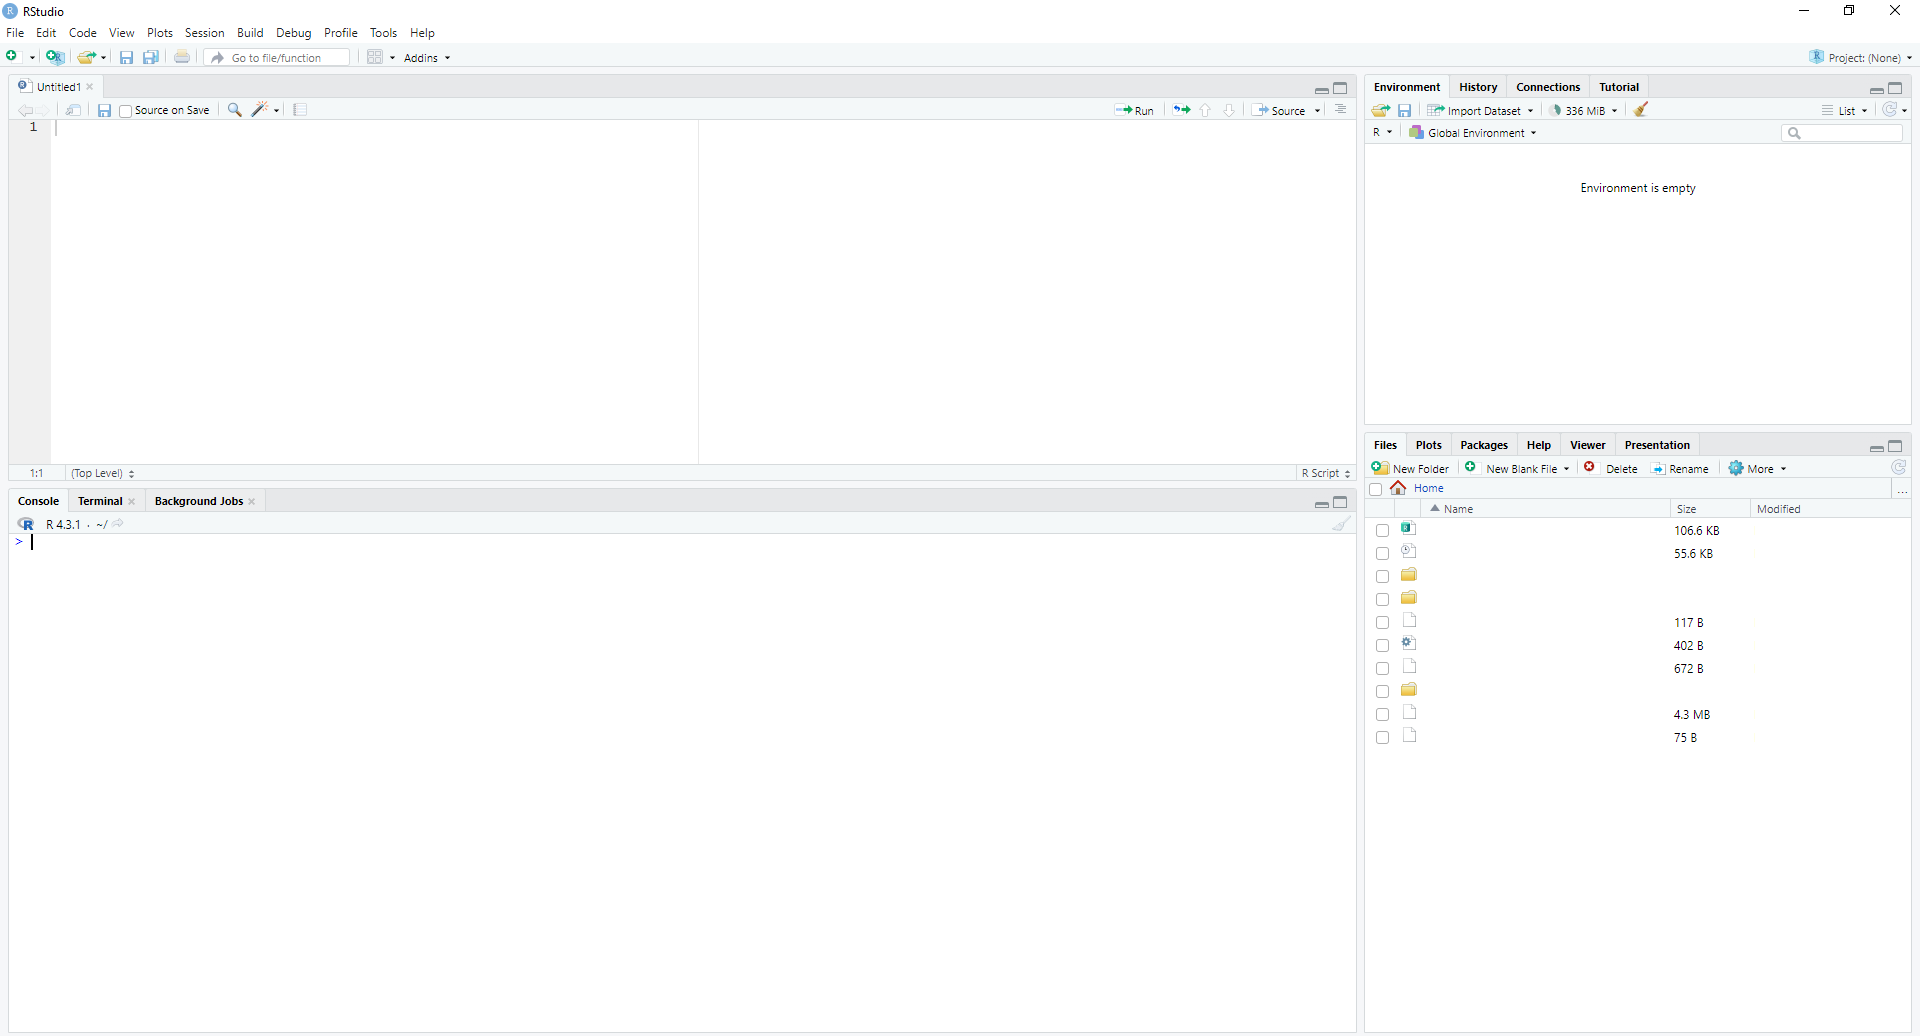
\includegraphics[width=0.7\linewidth]{images/imagen2.png}
\caption{\label{fig:rstudio_graphic_interface}Interfaz gráfica de RStudio}
\end{figure}

\item 
Primero vamos a revisar el menú de RStudio, situado en la parte superior izquierda de la ventana, con las siguientes opciones:

\begin{itemize}
    \item 
    En la opción File, podemos crear archivos de varias extensiones como R, Rnw, C, entre otros (New File); Podemos abrir también archivos, guardarlos, etc. También, podemos cargar sets de datos (Import dataset), por ejemplo en formato Excel, texto plano, etc.
    
    Además, podemos crear un proyecto (New Project) y abrirlo (Open Project). Para esta práctica, crearemos un nuevo proyecto. Podemos escoger si crear un directorio al crearlo, o crear el proyecto dentro de un directorio ya existente. Una vez lo creamos, el directorio de trabajo será el directorio en el que se encuentre nuestro proyecto, por lo que no tendremos que preocuparnos de establecer el directorio de trabajo manualmente.
    \item La opción Edit sirve para utilizarse con el panel de editor de textos, aunque no es muy utilizada si se usan atajos del teclado. La única opción interesante es la de Folding, con la cual podemos ocultar todo el contenido del ámbito de las funciones, para no tener que desplazarse hasta su final para ver el contenido por debajo de la misma.
    \item La opción Code sirve sobre todo para ejecutar archivos .R, aunque con el editor de textos no se utilizará mucho, ya que ya tiene incorporado un botón para hacer source con el archivo que actualmente se muestra en el editor de textos
    \item La opción View gestiona lo que se muestra en la interfaz gráfica. Una de sus opciones sirve para configurar los paneles que podemos observar, y a la cual accederemos más tarde
    \item La opción Plots sirve para gestionar el dibujado de los gráficos, y es importante si se van a utilizar.
    \item La opción Session sirve para gestionar cómo se ejecutan los procesos y subprocesos en R. No lo vamos a utilizar.
    \item La opción Build sirve para abrir una opción de una ventana de opciones que veremos más tarde, que no necesita ser accedida a través de esta opción
    \item La opción Debug nos servirá para encontrar bugs en nuestros archivos .R. Es posible que lo utilicemos
    \item La opción Profile podemos obtener información acerca del rendimiento de la ejecución de las funciones en R, entre otros. No nos va a hacer falta esta opción.
    \item La opción Tools podemos instalar y actualizar paquetes, aunque la interfaz gráfica ya tiene incorporada en uno de sus paneles esta opción, y acceder a opciones de configuración globales y de nuestro proyecto actual. Lo que si utilizaremos es su opción Global Options, con la cual podemos configurar todas las opciones de RStudio.
    \item La opción Help nos sirve para buscar ayuda acerca de cualquier paquete o función, aunque la interfaz gráfica ya tiene incorporada en uno de sus paneles esta opción, por lo cual apenas la vamos a utilizar
\end{itemize}

\item
Ahora vamos a comentar los paneles que podemos ver en la interfaz gráfica:

\begin{itemize}
\item
Podemos observar que en el panel de la esquina inferior derecha, podemos ver los archivos que están en el directorio de trabajo actual (Files), los gráficos que se dibujan por la ejecución del programa (Plots), todos los paquetes que podemos instalar y cargar (Packages, aunque nosotros utilizaremos la misma técnica vista en la práctica anterior), toda la descripción de alguna función o paquete del cual queramos obtener más información (Help), entre otros.
\item
En el panel de la esquina superior derecha podemos observar todas las variables que se van creando durante la ejecución de funciones en la consola (Environment), las líneas ejecutadas en la terminal (History), entre otros
\item
En el panel de la esquina inferior izquierda podemos observar la consola de ejecución de R (Console), una opción para iniciar una terminal en este panel (Terminal), entre otros
\item
En el panel de la esquina superior izquierda podemos observar el editor de archivos, que por defecto prepara un archivo de extensión .r llamado Untitled1.
\end{itemize}

\item 
Si abrimos la opción View -> Panes -> Pane Layout... podemos ver todos los paneles que podemos ver en la interfaz, y cada uno qué muestra. Podemos observar que los dos paneles a la izquierda son, arriba, "Source", y abajo, "Console". Podemos cambiar este orden seleccionando que el panel superior a la izquierda sea "Console". Una vez hecho, pulsamos el botón de aplicar, y ya habremos cambiado el orden
\begin{figure}[H]
\centering
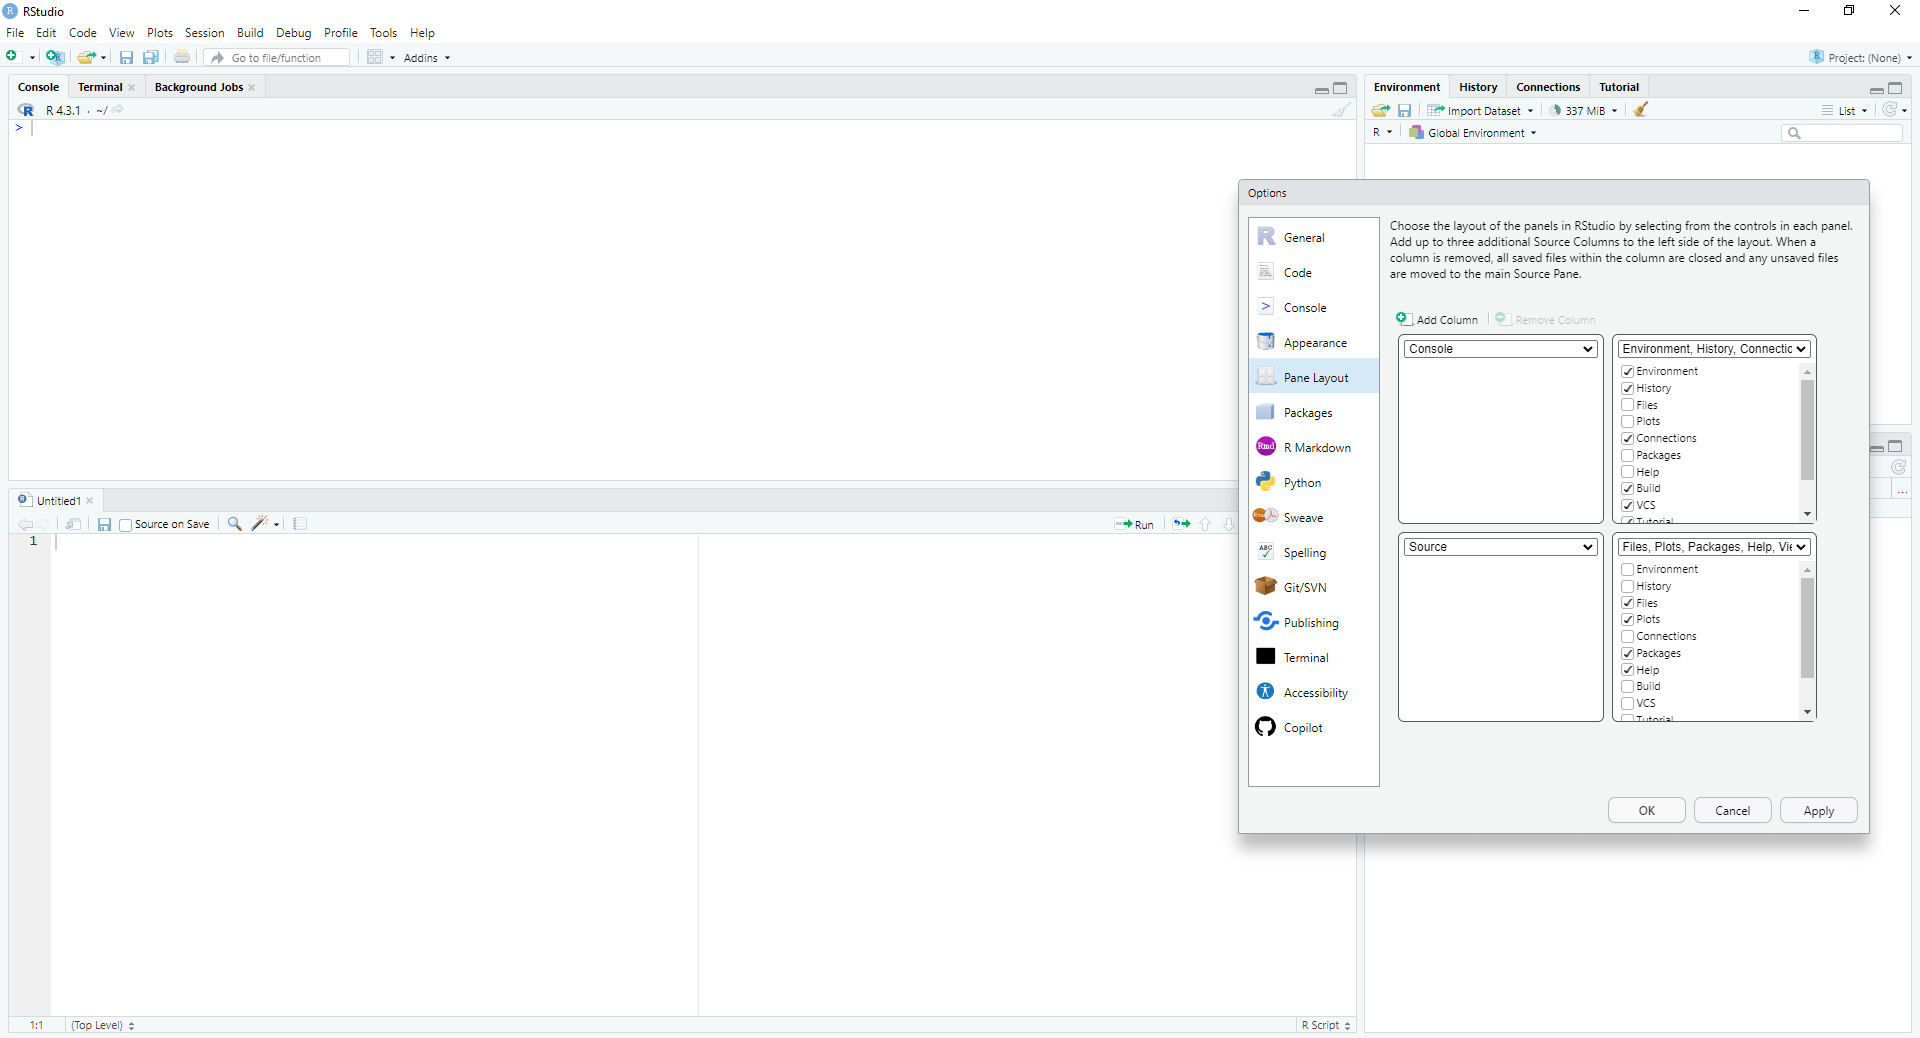
\includegraphics[width=0.7\linewidth]{images/imagen3.png}
\caption{\label{fig:rstudio_pane_layout}Opción Pane Layout}
\end{figure}

\item
En la ventana con el título Options que nos ha aparecido, también podemos configurar otras opciones. Podemos abrir la misma ventana pero con más opciones si nos dirigimos a la opción Tools -> Global options...

Con toda esta información, deberíamos ser capaces de empezar a trabajar con RStudio.

\end{enumerate}

\subsection{Explicación de la carga de tablas en formato Excel}

En todos los ejercicios de la parte 2 se explica brevemente cómo cargar los datos de los ejercicios que se van a utilizar en tablas cuyo formato es Excel (xslx), pero vamos a explicar cómo se hace esta carga antes de ver los ejercicios

Podemos encontrar este paquete en el siguiente enlace del repositorio de CRAN: \href{https://cran.rediris.es/web/packages/readxl/index.html}{Paquete readxl}. Descargamos el paquete, y lo cargamos como de costumbre (recordar guardar el archivo zip en el directorio tmp que creamos en C:):


\begin{Schunk}
\begin{Sinput}
> install.packages("C:/tmp/readxl_1.4.3.zip", repos=NULL)
\end{Sinput}
\end{Schunk}


Para utilizarlo, cargamos la librería


\begin{Schunk}
\begin{Sinput}
> library(readxl)
\end{Sinput}
\end{Schunk}


Y en teoría, ya podríamos utilizarlo. Por ejemplo, podemos cargar la tabla del ejercicio 1 de la parte 2:


\begin{Schunk}
\begin{Sinput}
> (fichero <- read_excel("Libro 1.xlsx"))
\end{Sinput}
\begin{Soutput}
# A tibble: 15 × 2
   Velocidad Temperatura
       <dbl>       <dbl>
 1      3.5         4.5 
 2      0.75        3.25
 3      0           3   
 4      1.75        0.75
 5      3           3.75
 6      3.75        4.5 
 7      1.25        0.75
 8      0.25        3   
 9      3.5         4.25
10      1.5         0.5 
11      1           1   
12      3           4   
13      0.5         3   
14      2           0.25
15      0           2.5 
\end{Soutput}
\end{Schunk}


\section{Parte 1}

En este ejercicio, vamos a comentar la resolución, vista en clase de laboratorio, de cada uno de los cuatro apartados de la práctica.

\subsection{Ejercicio 1.1}

En este primer enunciado nos piden realizar el análisis de clasificación no supervisada con K-means en un conjunto de datos que nos aporta el enunciado. Ahora vamos a ver la resolución paso a paso:

\begin{enumerate}
    \item Formamos la matriz con los datos que nos proporciona el enunciado, la siguiente línea nos servirá


\begin{Schunk}
\begin{Sinput}
> m <- matrix(c(4,4,3,5,1,2,5,5,0,1,2,2,4,5,2,1),2,8)
\end{Sinput}
\end{Schunk}


    Aun no hemos terminado, tenemos que realizar la traspuesta de la matriz realizada anteriormente, estos se realiza con la siguiente línea de código


\begin{Schunk}
\begin{Sinput}
> (m <- t(m))
\end{Sinput}
\begin{Soutput}
     [,1] [,2]
[1,]    4    4
[2,]    3    5
[3,]    1    2
[4,]    5    5
[5,]    0    1
[6,]    2    2
[7,]    4    5
[8,]    2    1
\end{Soutput}
\end{Schunk}


    \item Una vez tenemos la matriz con los datos, necesitamos seleccionar los centroides, en este caso los centroides que vamos a seleccionar son los vistos en clase de teoría:

    \begin{itemize}
        \item Centroide 1 cuya posición es (0,1).
        \item Centroide 2 cuya posición es (2,2).
    \end{itemize}

    Con los centroides seleccionados tenemos que hacer un tratamiento similar al de los datos, para ello utilizamos el siguiente código


\begin{Schunk}
\begin{Sinput}
> c <- matrix(c(0,1,2,2),2,2)
> (c <- t(c))
\end{Sinput}
\begin{Soutput}
     [,1] [,2]
[1,]    0    1
[2,]    2    2
\end{Soutput}
\end{Schunk}


    \item Con los datos ya estructurados aplicamos la función kmeans del paquete stats, utilizamos la siguiente línea


\begin{Schunk}
\begin{Sinput}
> (clasificacionns = (kmeans(m,c,4)))
\end{Sinput}
\begin{Soutput}
K-means clustering with 2 clusters of sizes 4, 4

Cluster means:
  [,1] [,2]
1 1.25 1.50
2 4.00 4.75

Clustering vector:
[1] 2 2 1 2 1 1 2 1

Within cluster sum of squares by cluster:
[1] 3.75 2.75
 (between_SS / total_SS =  84.8 %)

Available components:

[1] "cluster"      "centers"      "totss"        "withinss"     "tot.withinss"
[6] "betweenss"    "size"         "iter"         "ifault"      
\end{Soutput}
\end{Schunk}


    Donde el primer parámetro es la matriz con los datos, el segundo parámetro es la matriz con los centroides y el tercer parámetro número máximo de iteraciones que puede hacer.

    \item Con lo que hemos realizado hasta ahora tenemos, entre otras cosas, a que cluster pertenece cada punto pero nos interese tener cada punto en su cluster para poder trabajar con ellos, para hacer esto vamos a juntar la columna cluster de clasificacionns con la matriz de datos con la siguiente línea


\begin{Schunk}
\begin{Sinput}
> (m = cbind(clasificacionns$cluster,m))
\end{Sinput}
\begin{Soutput}
     [,1] [,2] [,3]
[1,]    2    4    4
[2,]    2    3    5
[3,]    1    1    2
[4,]    2    5    5
[5,]    1    0    1
[6,]    1    2    2
[7,]    2    4    5
[8,]    1    2    1
\end{Soutput}
\end{Schunk}


    \item Ahora separamos la matriz resultante del conjunto anterior en un subconjunto para los puntos pertenecientes al cluster 1 y otro subconjunto para los puntos pertenecientes al cluster 2. Para hacer esto vamos a usar lo siguiente


\begin{Schunk}
\begin{Sinput}
> mc1 = subset(m,m[,1]==1)
> mc2 = subset(m,m[,1]==2)
\end{Sinput}
\end{Schunk}


    Vamos a comprobar como quedan


\begin{Schunk}
\begin{Sinput}
> mc1
\end{Sinput}
\begin{Soutput}
     [,1] [,2] [,3]
[1,]    1    1    2
[2,]    1    0    1
[3,]    1    2    2
[4,]    1    2    1
\end{Soutput}
\begin{Sinput}
> mc2
\end{Sinput}
\begin{Soutput}
     [,1] [,2] [,3]
[1,]    2    4    4
[2,]    2    3    5
[3,]    2    5    5
[4,]    2    4    5
\end{Soutput}
\end{Schunk}


    \item Por último, vamos a quitar la columna que indica a que cluster pertenece cada punto usando lo siguiente


\begin{Schunk}
\begin{Sinput}
> (mc1=mc1[,-1])
\end{Sinput}
\begin{Soutput}
     [,1] [,2]
[1,]    1    2
[2,]    0    1
[3,]    2    2
[4,]    2    1
\end{Soutput}
\begin{Sinput}
> (mc2=mc2[,-1])
\end{Sinput}
\begin{Soutput}
     [,1] [,2]
[1,]    4    4
[2,]    3    5
[3,]    5    5
[4,]    4    5
\end{Soutput}
\end{Schunk}


\end{enumerate}

\subsection{Ejercicio 1.2}

En este apartado nos piden realizar el análisis de clasificación no supervisada con Clusterización Jerárquica Aglomerativa en un conjunto de datos que nos aporta el enunciado. Ahora vamos a realizar la resolución paso a paso:

\begin{enumerate}
    \item Descargar el archivo zip del paquete LearnClust, y abrirlo con install.packages, indicando que no lo descargamos de ningún repositorio con repos=NULL. Podemos encontrar el paquete LearnClust en este enlace: \href{https://cran.rediris.es/web/packages/LearnClust/index.html}{LearnClust}
    
    El paquete que hemos descargado lo guardamos en una carpeta C:/tmp, dentro de la raíz del disco. Ahora realizaremos la instalación con la siguiente línea


\begin{Schunk}
\begin{Sinput}
> install.packages("C:\\tmp\\LearnClust_1.1.zip",repos=NULL)
\end{Sinput}
\end{Schunk}
  

    Ahora lo cargamos con la siguiente línea


\begin{Schunk}
\begin{Sinput}
> library(LearnClust)
\end{Sinput}
\end{Schunk}


\item A veces puede ser necesario este paquete, el cual vamos a instalar y cargar directamente, sin descargar el archivo .zip del repositorio de CRAN:

\begin{Schunk}
\begin{Sinput}
> install.packages("magick")
> library(magick)
\end{Sinput}
\end{Schunk}


    \item Ahora que tenemos el paquete que vamos a utilizar vamos a introducir los datos usando las siguientes líneas


\begin{Schunk}
\begin{Sinput}
> m <- matrix(c(0.89,2.94, 4.36,5.21, 3.75,1.12, 6.25,3.14, 4.1,1.8, 3.9,4.27),2,6)
> (m <- t(m))
\end{Sinput}
\begin{Soutput}
     [,1] [,2]
[1,] 0.89 2.94
[2,] 4.36 5.21
[3,] 3.75 1.12
[4,] 6.25 3.14
[5,] 4.10 1.80
[6,] 3.90 4.27
\end{Soutput}
\end{Schunk}


    \item Como ya tenemos los datos vamos a ejecutar el algoritmo con la siguiente línea


\begin{Schunk}
\begin{Sinput}
> agglomerativeHC(m,"EUC","MIN")
\end{Sinput}
\begin{Soutput}
$dendrogram
Number of objects: 6 


$clusters
$clusters[[1]]
    X1   X2
1 0.89 2.94

$clusters[[2]]
    X1   X2
1 4.36 5.21

$clusters[[3]]
    X1   X2
1 3.75 1.12

$clusters[[4]]
    X1   X2
1 6.25 3.14

$clusters[[5]]
   X1  X2
1 4.1 1.8

$clusters[[6]]
   X1   X2
1 3.9 4.27

$clusters[[7]]
    X1   X2
1 3.75 1.12
2 4.10 1.80

$clusters[[8]]
    X1   X2
1 4.36 5.21
2 3.90 4.27

$clusters[[9]]
    X1   X2
1 3.75 1.12
2 4.10 1.80
3 4.36 5.21
4 3.90 4.27

$clusters[[10]]
    X1   X2
1 6.25 3.14
2 3.75 1.12
3 4.10 1.80
4 4.36 5.21
5 3.90 4.27

$clusters[[11]]
    X1   X2
1 0.89 2.94
2 6.25 3.14
3 3.75 1.12
4 4.10 1.80
5 4.36 5.21
6 3.90 4.27


$groupedClusters
  cluster1 cluster2
1        3        5
2        2        6
3        7        8
4        4        9
5        1       10
\end{Soutput}
\end{Schunk}


    Donde el primer parámetro es la matriz de datos, el segundo parámetro es el método para calcular la distancia y el tercer parámetro es el tipo de algoritmo para definir la distancia.

    Si quisiéramos ver el algoritmo paso a paso tenemos que usar la siguiente instrucción.


\begin{Schunk}
\begin{Sinput}
> agglomerativeHC.details(m,"EUC","MIN")
\end{Sinput}
\begin{Soutput}
[[1]]
     [,1] [,2] [,3]
[1,] 0.89 2.94    1

[[2]]
     [,1] [,2] [,3]
[1,] 4.36 5.21    1

[[3]]
     [,1] [,2] [,3]
[1,] 3.75 1.12    1

[[4]]
     [,1] [,2] [,3]
[1,] 6.25 3.14    1

[[5]]
     [,1] [,2] [,3]
[1,]  4.1  1.8    1

[[6]]
     [,1] [,2] [,3]
[1,]  3.9 4.27    1

         [,1]     [,2]      [,3]     [,4]      [,5]     [,6]
[1,] 0.000000 4.146541 3.3899853 5.363730 3.4064204 3.290745
[2,] 4.146541 0.000000 4.1352388 2.803034 3.4198977 1.046518
[3,] 3.389985 4.135239 0.0000000 3.214094 0.7647876 3.153569
[4,] 5.363730 2.803034 3.2140940 0.000000 2.5333969 2.607566
[5,] 3.406420 3.419898 0.7647876 2.533397 0.0000000 2.478084
[6,] 3.290745 1.046518 3.1535694 2.607566 2.4780839 0.000000
    X1   X2
1 3.75 1.12
2 4.10 1.80
         [,1]     [,2] [,3]     [,4] [,5]     [,6]     [,7]
[1,] 0.000000 4.146541    0 5.363730    0 3.290745 3.389985
[2,] 4.146541 0.000000    0 2.803034    0 1.046518 3.419898
[3,] 0.000000 0.000000    0 0.000000    0 0.000000 0.000000
[4,] 5.363730 2.803034    0 0.000000    0 2.607566 2.533397
[5,] 0.000000 0.000000    0 0.000000    0 0.000000 0.000000
[6,] 3.290745 1.046518    0 2.607566    0 0.000000 2.478084
[7,] 3.389985 3.419898    0 2.533397    0 2.478084 0.000000
    X1   X2
1 4.36 5.21
2 3.90 4.27
         [,1] [,2] [,3]     [,4] [,5] [,6]     [,7]     [,8]
[1,] 0.000000    0    0 5.363730    0    0 3.389985 3.290745
[2,] 0.000000    0    0 0.000000    0    0 0.000000 0.000000
[3,] 0.000000    0    0 0.000000    0    0 0.000000 0.000000
[4,] 5.363730    0    0 0.000000    0    0 2.533397 2.607566
[5,] 0.000000    0    0 0.000000    0    0 0.000000 0.000000
[6,] 0.000000    0    0 0.000000    0    0 0.000000 0.000000
[7,] 3.389985    0    0 2.533397    0    0 0.000000 2.478084
[8,] 3.290745    0    0 2.607566    0    0 2.478084 0.000000
    X1   X2
1 3.75 1.12
2 4.10 1.80
3 4.36 5.21
4 3.90 4.27
          [,1] [,2] [,3]     [,4] [,5] [,6] [,7] [,8]     [,9]
 [1,] 0.000000    0    0 5.363730    0    0    0    0 3.290745
 [2,] 0.000000    0    0 0.000000    0    0    0    0 0.000000
 [3,] 0.000000    0    0 0.000000    0    0    0    0 0.000000
 [4,] 5.363730    0    0 0.000000    0    0    0    0 2.533397
 [5,] 0.000000    0    0 0.000000    0    0    0    0 0.000000
 [6,] 0.000000    0    0 0.000000    0    0    0    0 0.000000
 [7,] 0.000000    0    0 0.000000    0    0    0    0 0.000000
 [8,] 0.000000    0    0 0.000000    0    0    0    0 0.000000
 [9,] 3.290745    0    0 2.533397    0    0    0    0 0.000000
    X1   X2
1 6.25 3.14
2 3.75 1.12
3 4.10 1.80
4 4.36 5.21
5 3.90 4.27
          [,1] [,2] [,3] [,4] [,5] [,6] [,7] [,8] [,9]    [,10]
 [1,] 0.000000    0    0    0    0    0    0    0    0 3.290745
 [2,] 0.000000    0    0    0    0    0    0    0    0 0.000000
 [3,] 0.000000    0    0    0    0    0    0    0    0 0.000000
 [4,] 0.000000    0    0    0    0    0    0    0    0 0.000000
 [5,] 0.000000    0    0    0    0    0    0    0    0 0.000000
 [6,] 0.000000    0    0    0    0    0    0    0    0 0.000000
 [7,] 0.000000    0    0    0    0    0    0    0    0 0.000000
 [8,] 0.000000    0    0    0    0    0    0    0    0 0.000000
 [9,] 0.000000    0    0    0    0    0    0    0    0 0.000000
[10,] 3.290745    0    0    0    0    0    0    0    0 0.000000
    X1   X2
1 0.89 2.94
2 6.25 3.14
3 3.75 1.12
4 4.10 1.80
5 4.36 5.21
6 3.90 4.27
\end{Soutput}
\end{Schunk}


    \item Vamos a hacer lo mismo pero con MAX. En este caso solo tenemos que realizar un cambio.


\begin{Schunk}
\begin{Sinput}
> agglomerativeHC(m,"EUC","MAX")
\end{Sinput}
\begin{Soutput}
$dendrogram
Number of objects: 6 


$clusters
$clusters[[1]]
    X1   X2
1 0.89 2.94

$clusters[[2]]
    X1   X2
1 4.36 5.21

$clusters[[3]]
    X1   X2
1 3.75 1.12

$clusters[[4]]
    X1   X2
1 6.25 3.14

$clusters[[5]]
   X1  X2
1 4.1 1.8

$clusters[[6]]
   X1   X2
1 3.9 4.27

$clusters[[7]]
    X1   X2
1 3.75 1.12
2 4.10 1.80

$clusters[[8]]
    X1   X2
1 4.36 5.21
2 3.90 4.27

$clusters[[9]]
    X1   X2
1 6.25 3.14
2 4.36 5.21
3 3.90 4.27

$clusters[[10]]
    X1   X2
1 0.89 2.94
2 3.75 1.12
3 4.10 1.80

$clusters[[11]]
    X1   X2
1 6.25 3.14
2 4.36 5.21
3 3.90 4.27
4 0.89 2.94
5 3.75 1.12
6 4.10 1.80


$groupedClusters
  cluster1 cluster2
1        3        5
2        2        6
3        4        8
4        1        7
5        9       10
\end{Soutput}
\begin{Sinput}
> agglomerativeHC.details(m,"EUC","MAX")
\end{Sinput}
\begin{Soutput}
[[1]]
     [,1] [,2] [,3]
[1,] 0.89 2.94    1

[[2]]
     [,1] [,2] [,3]
[1,] 4.36 5.21    1

[[3]]
     [,1] [,2] [,3]
[1,] 3.75 1.12    1

[[4]]
     [,1] [,2] [,3]
[1,] 6.25 3.14    1

[[5]]
     [,1] [,2] [,3]
[1,]  4.1  1.8    1

[[6]]
     [,1] [,2] [,3]
[1,]  3.9 4.27    1

         [,1]     [,2]      [,3]     [,4]      [,5]     [,6]
[1,] 0.000000 4.146541 3.3899853 5.363730 3.4064204 3.290745
[2,] 4.146541 0.000000 4.1352388 2.803034 3.4198977 1.046518
[3,] 3.389985 4.135239 0.0000000 3.214094 0.7647876 3.153569
[4,] 5.363730 2.803034 3.2140940 0.000000 2.5333969 2.607566
[5,] 3.406420 3.419898 0.7647876 2.533397 0.0000000 2.478084
[6,] 3.290745 1.046518 3.1535694 2.607566 2.4780839 0.000000
    X1   X2
1 3.75 1.12
2 4.10 1.80
         [,1]     [,2] [,3]     [,4] [,5]     [,6]     [,7]
[1,] 0.000000 4.146541    0 5.363730    0 3.290745 3.406420
[2,] 4.146541 0.000000    0 2.803034    0 1.046518 4.135239
[3,] 0.000000 0.000000    0 0.000000    0 0.000000 0.000000
[4,] 5.363730 2.803034    0 0.000000    0 2.607566 3.214094
[5,] 0.000000 0.000000    0 0.000000    0 0.000000 0.000000
[6,] 3.290745 1.046518    0 2.607566    0 0.000000 3.153569
[7,] 3.406420 4.135239    0 3.214094    0 3.153569 0.000000
    X1   X2
1 4.36 5.21
2 3.90 4.27
         [,1] [,2] [,3]     [,4] [,5] [,6]     [,7]     [,8]
[1,] 0.000000    0    0 5.363730    0    0 3.406420 4.146541
[2,] 0.000000    0    0 0.000000    0    0 0.000000 0.000000
[3,] 0.000000    0    0 0.000000    0    0 0.000000 0.000000
[4,] 5.363730    0    0 0.000000    0    0 3.214094 2.803034
[5,] 0.000000    0    0 0.000000    0    0 0.000000 0.000000
[6,] 0.000000    0    0 0.000000    0    0 0.000000 0.000000
[7,] 3.406420    0    0 3.214094    0    0 0.000000 4.135239
[8,] 4.146541    0    0 2.803034    0    0 4.135239 0.000000
    X1   X2
1 6.25 3.14
2 4.36 5.21
3 3.90 4.27
         [,1] [,2] [,3] [,4] [,5] [,6]     [,7] [,8]     [,9]
 [1,] 0.00000    0    0    0    0    0 3.406420    0 5.363730
 [2,] 0.00000    0    0    0    0    0 0.000000    0 0.000000
 [3,] 0.00000    0    0    0    0    0 0.000000    0 0.000000
 [4,] 0.00000    0    0    0    0    0 0.000000    0 0.000000
 [5,] 0.00000    0    0    0    0    0 0.000000    0 0.000000
 [6,] 0.00000    0    0    0    0    0 0.000000    0 0.000000
 [7,] 3.40642    0    0    0    0    0 0.000000    0 4.135239
 [8,] 0.00000    0    0    0    0    0 0.000000    0 0.000000
 [9,] 5.36373    0    0    0    0    0 4.135239    0 0.000000
    X1   X2
1 0.89 2.94
2 3.75 1.12
3 4.10 1.80
      [,1] [,2] [,3] [,4] [,5] [,6] [,7] [,8]    [,9]   [,10]
 [1,]    0    0    0    0    0    0    0    0 0.00000 0.00000
 [2,]    0    0    0    0    0    0    0    0 0.00000 0.00000
 [3,]    0    0    0    0    0    0    0    0 0.00000 0.00000
 [4,]    0    0    0    0    0    0    0    0 0.00000 0.00000
 [5,]    0    0    0    0    0    0    0    0 0.00000 0.00000
 [6,]    0    0    0    0    0    0    0    0 0.00000 0.00000
 [7,]    0    0    0    0    0    0    0    0 0.00000 0.00000
 [8,]    0    0    0    0    0    0    0    0 0.00000 0.00000
 [9,]    0    0    0    0    0    0    0    0 0.00000 5.36373
[10,]    0    0    0    0    0    0    0    0 5.36373 0.00000
    X1   X2
1 6.25 3.14
2 4.36 5.21
3 3.90 4.27
4 0.89 2.94
5 3.75 1.12
6 4.10 1.80
\end{Soutput}
\end{Schunk}
  

    \item Con la siguiente instrucción mostramos un gráfico que representa la jerarquía de clusters.


\begin{Schunk}
\begin{Sinput}
> cmax <- agglomerativeHC(m,"EUC","MAX")
> plot(cmax$dendrogram)
\end{Sinput}
\end{Schunk}
\includegraphics{Grupo.5-PL2-n1_2_7}


    El gráfico que se mostraría sería el siguiente:
    \begin{figure}
        \centering
        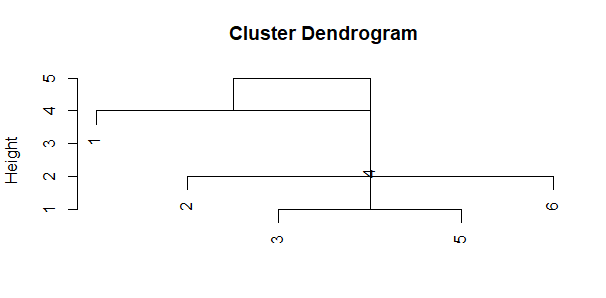
\includegraphics[width=0.5\linewidth]{images/imagen4.png}
        \caption{Gráfico}
        \label{fig:enter-label}
    \end{figure}
\end{enumerate}

\subsection{Ejercicio 1.3}

Para este apartado, describiremos los pasos realizados en laboratorio para resolver un problema de clasificación supervisada utilizando árboles de decisión.

Lo primero que debemos hacer es descargar el paquete \textbf{rpart}, el cual se encarga de hacer la clasificación supervisada por medio de un árbol de decisión. Esta librería se puede descargar en la siguiente dirección: \href{https://cran.r-project.org/web/packages/rpart/index.html}{paquete rpart}

Lo instalamos:


\begin{Schunk}
\begin{Sinput}
> install.packages("C:\\tmp\\rpart_4.1.23.zip",repos=NULL)
\end{Sinput}
\end{Schunk}


Y lo cargamos:


\begin{Schunk}
\begin{Sinput}
> library(rpart)
\end{Sinput}
\end{Schunk}


Para realizar esta clasificación, primero guardaremos los datos en un fichero de texto llamado 'Calificaciones.txt'. 

Este fichero tendrá 5 columnas separadas por tabulaciones, y dichas columnas serán la numeración de las filas, la nota de teoría, la nota de prácticas, la nota de laboratorio y la calificación general, siendo esta última la que queremos clasificar. 

\begin{figure}[H]
\centering
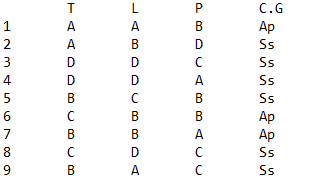
\includegraphics[width=0.7\linewidth]{images/imagen5.png}
\caption{\label{fig:tabla_calificaciones}Tabla Calificaciones.txt}
\end{figure}

Tras realizar el archivo de datos, este será importado a R con el comando read.table, guardando los datos en la variable clasificaciones.


\begin{Schunk}
\begin{Sinput}
> calificaciones = read.table("Calificaciones.txt")
\end{Sinput}
\end{Schunk}


Posteriormente, como queremos guardar los datos en forma de data frame, realizaremos una conversion mediante el comando data.frame('calificaciones') y mostraremos el resultado por pantalla.


\begin{Schunk}
\begin{Sinput}
> (muestra=data.frame(calificaciones))
\end{Sinput}
\begin{Soutput}
  T L P C.G
1 A A B  Ap
2 A B D  Ss
3 D D C  Ss
4 D D A  Ss
5 B C B  Ss
6 C B B  Ap
7 B B A  Ap
8 C D C  Ss
9 B A C  Ss
\end{Soutput}
\end{Schunk}


Por ultimo, usaremos el comando rpart para realizar la clasificación supervisada. Este comando utilizará 4 parámetros los cuales explicaremos a continuación.

\begin{enumerate}

\item
El primer parámetro será el valor que queramos clasificar, seguido de una virgulilla (\textasciitilde{}) y el nombre de las demás columnas que servirán para realizar la clasificación, separados por el símbolo más ('+'). En nuestro caso, como queremos clasificar la columna 'C.G', así que este parámetro será 'C.G \textasciitilde{} T+L+P'.

\item
El segundo parámetro es sobre que datos queremos actuar. En nuestro caso, queremos actuar sobre los datos de muestra, así que nuestro segundo parámetro será data=muestra.

\item
Para el tercer parámetro, utilizaremos el method=class ya que nuestro resultado viene dado por un conjunto de factores (notas de teoría, práctica y laboratorio).

\item
Por último, para nuestro ultimo parámetro debemos marcar el número mínimo de observaciones que deben existir en un nodo para que la división tenga éxito. Como nos interesa que se dividan aunque solo haya un elemento, pondremos minsplit=1

\end{enumerate}

Así entonces la linea final de nuestro código será la siguiente:


\begin{Schunk}
\begin{Sinput}
> clasificaciones = rpart(C.G~T+L+P,data=muestra, method="class",minsplit=1)
\end{Sinput}
\end{Schunk}


Cuya salida será:


\begin{Schunk}
\begin{Sinput}
> clasificaciones
\end{Sinput}
\begin{Soutput}
n= 9 

node), split, n, loss, yval, (yprob)
      * denotes terminal node

1) root 9 3 Ss (0.3333333 0.6666667)  
  2) L=A,B 5 2 Ap (0.6000000 0.4000000)  
    4) P=A,B 3 0 Ap (1.0000000 0.0000000) *
    5) P=C,D 2 0 Ss (0.0000000 1.0000000) *
  3) L=C,D 4 0 Ss (0.0000000 1.0000000) *
\end{Soutput}
\end{Schunk}


\subsection{Ejercicio 1.4}

En este último apartado se nos pide una clasificación supervisada utilizando regresión.
Para ello, primero estructuraremos los datos en un .txt, con el nombre del planeta, su radio y su densidad. A este fichero lo llamaremos planetas.txt.

Como es habitual, lo cargaremos en R utilizando el comando read.table, y al resultado de la importación lo llamaremos planetas.

\begin{figure}[H]
\centering
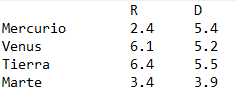
\includegraphics[width=0.7\linewidth]{images/imagen6.png}
\caption{\label{fig:tabla_planetas}Tabla planetas.txt}
\end{figure}


\begin{Schunk}
\begin{Sinput}
> planetas = read.table("planetas.txt")
\end{Sinput}
\end{Schunk}


Posteriormente, utilizaremos el comando lm que necesitará como parámetros la variable que queremos clasificar y aquella que nos proporciona dicha clasificación, separados por el símbolo \textasciitilde{}, y el nombre de la variable donde se encuentren los datos (en nuestro caso, planetas)


\begin{Schunk}
\begin{Sinput}
> regresion=lm(D~R, data=planetas)
> regresion
\end{Sinput}
\begin{Soutput}
Call:
lm(formula = D ~ R, data = planetas)

Coefficients:
(Intercept)            R  
     4.3624       0.1394  
\end{Soutput}
\end{Schunk}


Seguido de esto, podemos observar como la recta de regresión se ajusta a los puntos que tenemos mediante el comando summary, concretamente en su columna residuals. Esto nos servirá para identificar posibles outliers, ya que esta columna nos permite ver la distancia entre el punto y la recta.


\begin{Schunk}
\begin{Sinput}
> res = summary(regresion)$residuals
\end{Sinput}
\end{Schunk}


Por último, procederemos a calcular la desviación típica del conjunto para posteriormente localizar outliers mediante un bucle for.


\begin{Schunk}
\begin{Sinput}
> sr=sqrt(sum(res^2)/4)
> for (i in 1:length(res)){
+   if(res[i]>3*sr){
+     print("El suceso ");print(res[i]);print(" es un outlier")
+   }
+ }
\end{Sinput}
\end{Schunk}


En este caso, no encontramos ningún outlier

\section{Parte 2}

En esta parte, vamos a repetir los ejercicios anteriores, pero utilizaremos datos diferentes y propondremos una forma de solucionarlos distinta a la vista en clase.

\subsection{Ejercicio 2.1}

En este ejercicio nos piden realizar un análisis de clasificación no supervisada con K-means en un conjunto de datos. Dicho conjunto de datos se encuentra en un fichero excel entonces tendremos que cargarlos antes de hacer cualquier cosa.

Para cargar los datos haremos uso del paquete readxl. Ya que hemos explicado cómo instalarlo, cargarlo y utilizarlo, directamente cargaremos los datos:


\begin{Schunk}
\begin{Sinput}
> (fichero_datos <- read_excel("Libro 2.xlsx"))
\end{Sinput}
\begin{Soutput}
# A tibble: 8 × 2
  Teoría Laboratorio
   <dbl>       <dbl>
1      4           4
2      3           5
3      1           2
4      5           5
5      0           1
6      2           2
7      4           5
8      2           1
\end{Soutput}
\begin{Sinput}
> (fichero_centroides <- read_excel("Libro 3.xlsx"))
\end{Sinput}
\begin{Soutput}
# A tibble: 2 × 2
  `Posicion X` `Posicion Y`
         <dbl>        <dbl>
1            0            1
2            2            2
\end{Soutput}
\end{Schunk}


Aunque tengamos los datos, aun tenemos que prepararlos para que el algoritmo K-means que hemos programado para ello utilizaremos la siguiente función.


\begin{Schunk}
\begin{Sinput}
> preparar_datos <-
+ function(datos_fichero){
+ 
+ # Creamos una lista vacia que contendrá todos los elementos
+ lista1 <- list()
+ 
+ # Recorremos todas las filas
+ for (fila in 1:longitud(datos_fichero [[1]])){
+   
+   # Creamos una lista vacia por fila
+   lista2 <- list()
+   
+   # Recorremos todas las columnas
+   for (columna in 1:longitud(datos_fichero)){
+     
+     # Metemos todos que se encuentran en la misma fila
+     lista2 [[longitud(lista2)+1]] <- datos_fichero[[columna]][[fila]]
+     
+   }
+   
+   # Metemos la lista que contiene todos los elementos de la misma fila
+   lista1[[longitud(lista1)+1]] <- lista2
+ }
+ 
+ return(lista1)
+ }
\end{Sinput}
\end{Schunk}


Donde le parámetro que le pasamos son los datos leídos del excel. La función anterior emplea, al igual que otras funciones, una función para calcular la longitud.


\begin{Schunk}
\begin{Sinput}
> longitud <- 
+   function (datos){
+     
+     contador <- 0
+     
+     # Recorremos todos los elementos sumando +1 por cada elemento
+     for (elemento in datos){
+     contador <- contador + 1
+     }
+     return (contador)
+ }
\end{Sinput}
\end{Schunk}


    Donde el único parámetro es el conjunto de datos del cual queremos saber la longitud. Esta función devuelve el número de elementos que tiene el conjunto que pasamos como parámetro.


\begin{Schunk}
\begin{Sinput}
> (longitud(list(1,2,3,4,5,6,7)))
\end{Sinput}
\begin{Soutput}
[1] 7
\end{Soutput}
\end{Schunk}

   
Ahora vamos a preparar los datos para utilizarlos empleando las siguientes instrucciones.


\begin{Schunk}
\begin{Sinput}
> (datos <- preparar_datos(fichero_datos))
\end{Sinput}
\begin{Soutput}
[[1]]
[[1]][[1]]
[1] 4

[[1]][[2]]
[1] 4


[[2]]
[[2]][[1]]
[1] 3

[[2]][[2]]
[1] 5


[[3]]
[[3]][[1]]
[1] 1

[[3]][[2]]
[1] 2


[[4]]
[[4]][[1]]
[1] 5

[[4]][[2]]
[1] 5


[[5]]
[[5]][[1]]
[1] 0

[[5]][[2]]
[1] 1


[[6]]
[[6]][[1]]
[1] 2

[[6]][[2]]
[1] 2


[[7]]
[[7]][[1]]
[1] 4

[[7]][[2]]
[1] 5


[[8]]
[[8]][[1]]
[1] 2

[[8]][[2]]
[1] 1
\end{Soutput}
\begin{Sinput}
> (centroides <- preparar_datos(fichero_centroides))
\end{Sinput}
\begin{Soutput}
[[1]]
[[1]][[1]]
[1] 0

[[1]][[2]]
[1] 1


[[2]]
[[2]][[1]]
[1] 2

[[2]][[2]]
[1] 2
\end{Soutput}
\end{Schunk}


Ahora que ya tenemos los datos podemos realizar K-means utilizando la siguiente función.


\begin{Schunk}
\begin{Sinput}
> algoritmok_means <- 
+ function (datos,centroides){
+ 
+ # realizamos la primera iteración
+ # formación de la matriz de distancias
+ matriz_distancias <- calcular_matriz_distancias(datos,centroides)
+ 
+ # formación de la matriz de pertenencia
+ matriz_pertenencia <- calcular_matriz_pertenencia(datos,centroides,matriz_distancias)
+ 
+ # pasamos a la siguiente iteración
+ siguiente_iteracion(datos, matriz_pertenencia)
+ 
+ }
\end{Sinput}
\end{Schunk}


Donde el primer parámetro que le pasamos son los datos y el segundo parámetro los centroides. Antes de ver el resultado vamos a ver paso a paso su funcionamiento:

\begin{itemize}
    \item El primer paso es realizar la primera iteración del algoritmo K-means, para ello utilizaremos las siguientes funciones.


\begin{Schunk}
\begin{Sinput}
> calcular_matriz_distancias <- 
+ function(datos,centroides){
+ 
+ # Crearemos la matriz llena de ceros
+ matriz_distancias <- array (0, dim = c(longitud(centroides),longitud(datos)))
+ 
+ # Calculamos la distancia euclidea de los puntos a los centroides y los 
+ # guardamos en la matriz
+ for (i in 1:longitud(datos)){
+ for (j in 1:longitud(centroides)){
+ distancia <- 
+ sqrt((centroides[[j]][[1]] - datos[[i]][[1]])^2 + 
+ (centroides[[j]][[2]] - datos[[i]][[2]])^2)
+ matriz_distancias[j,i] <- distancia
+ }
+ }
+ 
+ return(matriz_distancias)
+ }
\end{Sinput}
\end{Schunk}


    Donde el primer parámetro es la posición de los puntos y el segundo parámetro la posición de los centroides.Haciendo uso de esta función obtendremos una matriz con la distancia de los puntos a los centroides.

    Un ejemplo de la función para calcular la matriz distancia sería el siguiente.


\begin{Schunk}
\begin{Sinput}
>     (matriz_distancias <- calcular_matriz_distancias(datos,centroides))
\end{Sinput}
\begin{Soutput}
         [,1]     [,2]     [,3]     [,4]     [,5]     [,6]     [,7] [,8]
[1,] 5.000000 5.000000 1.414214 6.403124 0.000000 2.236068 5.656854    2
[2,] 2.828427 3.162278 1.000000 4.242641 2.236068 0.000000 3.605551    1
\end{Soutput}
\end{Schunk}


    Después de calcular la matriz de distancias tenemos que asignar los puntos a los centroides, para ello utilizaremos la siguiente función.


\begin{Schunk}
\begin{Sinput}
> calcular_matriz_pertenencia <- 
+ function(datos,centroides,matriz_distancias){
+ 
+ # Creamos la matriz llena de ceros
+ matriz_pertenencia <- array (0, dim = c(longitud(centroides),longitud(datos)))
+ 
+ # Miramos de cada punto a que centroide está más cerca
+ for (i in 1:longitud(datos)){
+ distancias_al_punto <- list()
+ for (j in 1:longitud(centroides)){
+ distancias_al_punto[[longitud(distancias_al_punto) + 1]] <- matriz_distancias[j,i]
+ }
+ centroide_asignado <- posicion_minimo(distancias_al_punto)
+ matriz_pertenencia[centroide_asignado,i] <- 1
+ }
+     
+     return(matriz_pertenencia)
+ }
\end{Sinput}
\end{Schunk}


    Donde el primer parámetro es la posición de los puntos, el segundo parámetro la posición de los centroides y el tercer parámetro es la matriz de distancias. Esta función asignara los puntos a los centroides más cercanos.

    Para realizar esto tenemos que utilizar la función longitud y posición mínima. Esta última sería así.


\begin{Schunk}
\begin{Sinput}
> posicion_minimo <-
+ function(datos){
+ 
+ # Iniciliazamos la posicion donde se encuentra el valor mínimo
+ pos_min <- 1
+ 
+ # Inicializar el mínimo con el primer elemento del array
+ minimo_valor <- datos[1]
+ 
+ # Iterar sobre los elementos del array para encontrar el mínimo
+ for (i in 2:longitud(datos)) {
+ valor <- datos[[i]]
+ 
+ if (valor < minimo_valor) {
+     minimo_valor <- valor
+     pos_min <- i
+ }
+ }
+ 
+ return(pos_min)
+ }
\end{Sinput}
\end{Schunk}


    Donde el único parámetro es un conjuntos de datos. Esta función devuelve la posición donde se encuentra el valor más pequeño del conjunto de datos. Un ejemplo de su funcionamientos sería.


\begin{Schunk}
\begin{Sinput}
>     (posicion_minimo(list(1,2,3,4,0.5,6,7,8)))
\end{Sinput}
\begin{Soutput}
[1] 5
\end{Soutput}
\end{Schunk}


    Un ejemplo de la salida de la función para calcular la matriz de pertenencia seria el siguiente.


\begin{Schunk}
\begin{Sinput}
>     (matriz_pertenencia 
+     <- calcular_matriz_pertenencia(datos,centroides,matriz_distancias))
\end{Sinput}
\begin{Soutput}
     [,1] [,2] [,3] [,4] [,5] [,6] [,7] [,8]
[1,]    0    0    0    0    1    0    0    0
[2,]    1    1    1    1    0    1    1    1
\end{Soutput}
\end{Schunk}


    Con esto ya habríamos acabado la primera iteración del algoritmo K-means. Ahora vamos a realizar la segunda parte del algoritmo K-means, que consiste en calcular los nuevos centroides, calcular las distancias de los puntos a los centroides y asignar los puntos hasta que la asignación no de los puntos sean iguales en dos iteraciones consecutivas. Para esto vamos a usar la siguiente función.


\begin{Schunk}
\begin{Sinput}
> siguiente_iteracion <-
+ function(datos,matriz_pertenencia_antigua){
+ 
+ # inicializamos los centroides
+ centroides <- list()
+ 
+ # calculamos los nuevos centroides
+ for (i in 1:dim(matriz_pertenencia_antigua)[1]){
+ x <- 0
+ y <- 0
+ pertenecientes <- 0
+ nuevo_centroide <- list()
+ 
+ for (j in 1:dim(matriz_pertenencia_antigua)[2]){
+ if(matriz_pertenencia_antigua[i,j] == 1){
+ x <- x + datos[[j]][[1]]
+ y <- y + datos[[j]][[2]]
+ pertenecientes <- pertenecientes + 1
+ }
+ }
+ 
+ nuevo_centroide[longitud(nuevo_centroide)+1] <- (x/pertenecientes)
+ nuevo_centroide[longitud(nuevo_centroide)+1] <- (y/pertenecientes)
+ 
+ centroides[longitud(centroides)+1] <- list(nuevo_centroide)
+ 
+ }
+ 
+ # formación de la matriz de distancias
+ matriz_distancias <- calcular_matriz_distancias(datos,centroides)
+ 
+ # formación de la matriz de pertenencia
+ matriz_pertenencia <- calcular_matriz_pertenencia(datos
+ ,centroides,matriz_distancias)
+ 
+ # miramos si la matriz de pertenencia ha sufrido cambios
+ if(!matrices_iguales(matriz_pertenencia,matriz_pertenencia_antigua)){
+ siguiente_iteracion(datos,matriz_pertenencia)
+ }else{
+ 
+ clusters <- list()
+ 
+ # formamos los clusters
+ for (fila in 1:dim(matriz_pertenencia)[1]){
+ 
+ cat("\n\nEl cluster",fila,"tiene el centroide en",centroides[[fila]][[1]],","
+ ,centroides[[fila]][[2]],"\n")
+ 
+ cluster_nuevo <- list()
+ 
+ cat("Y esta formado por:\n")
+ 
+ for (columna in 1:dim(matriz_pertenencia)[2]){
+ 
+ if (matriz_pertenencia[fila,columna]==1){
+     
+     cat("El punto",columna,"cuya posicion es",datos[[columna]][[1]],","
+     ,datos[[columna]][[2]],"\n")
+     
+     cluster_nuevo <- append(cluster_nuevo,datos[[columna]])
+     
+ }
+ 
+ }
+ 
+ matriz <- array(0, dim= c(longitud(cluster_nuevo)/2, 2))
+ 
+ for (dato in 1:longitud(cluster_nuevo)){
+ if (dato %% 2 == 0){
+     matriz[dato/2,2] <- cluster_nuevo[[dato]]
+ }
+ else{
+     matriz[floor(dato/2)+1,1] <- cluster_nuevo[[dato]]
+ }
+ }
+ 
+ clusters[longitud(clusters)+1] <- list(matriz)
+ 
+ }
+ 
+ return(clusters)
+ }
+ 
+ }
\end{Sinput}
\end{Schunk}


    Donde el primer parámetro es el conjunto de datos sobre el cual realizamos el análisis y el segundo parámetro es la matriz de pertenencia realizada en la iteración anterior. Como esta función es extensa vamos a ver que hace:

\begin{itemize}
    \item Primero tenemos que calcular la posición de los nuevos centroides, para realizar esto usamos el siguiente fragmento de código.


\begin{Schunk}
\begin{Sinput}
> # inicializamos los centroides
> centroides <- list()
> # calculamos los nuevos centroides
> for (i in 1:dim(matriz_pertenencia_antigua)[1]){
+ x <- 0
+ y <- 0
+ pertenecientes <- 0
+ nuevo_centroide <- list()
+ 
+ for (j in 1:dim(matriz_pertenencia_antigua)[2]){
+     if(matriz_pertenencia_antigua[i,j] == 1){
+     x <- x + datos[[j]][[1]]
+     y <- y + datos[[j]][[2]]
+     pertenecientes <- pertenecientes + 1
+     }
+ }
+ 
+ nuevo_centroide[longitud(nuevo_centroide)+1] <- (x/pertenecientes)
+ nuevo_centroide[longitud(nuevo_centroide)+1] <- (y/pertenecientes)
+ 
+ centroides[longitud(centroides)+1] <- list(nuevo_centroide)
+ 
+ }
\end{Sinput}
\end{Schunk}


    Para calcular la posición de los nuevos centroides miramos que puntos se le han asignado y calculamos la media de las coordenadas de los puntos que se le han asignado. 

    Con los centroides calculados, tenemos que calcular de nuevo la distancia de cada punto a los nuevos centroides y, posteriormente, asignarlos al centroide más próximo. Para realizar estos dos pasos usamos funciones anteriormente dichas.


\begin{Schunk}
\begin{Sinput}
> # formación de la matriz de distancias
> matriz_distancias <- calcular_matriz_distancias(datos,centroides)
> # formación de la matriz de pertenencia
> matriz_pertenencia <- calcular_matriz_pertenencia(datos,centroides
+ ,matriz_distancias)
\end{Sinput}
\end{Schunk}


    Con la nueva matriz de pertenencia, miramos si ha habido algún cambio en al asignación de los puntos respecto a la iteración anterior. Si ha habido un cambio en la asignación de puntos tenemos que realizar otra iteración, si no formaremos los clusters con los puntos a los que pertenecen, para que puedan trabajar en ellos, y mostraremos la composición de cada cluster. Para ello utilizaremos el siguiente fragmento de código.


\begin{Schunk}
\begin{Sinput}
> # miramos si la matriz de pertenencia ha sufrido cambios
> if(!matrices_iguales(matriz_pertenencia,matriz_pertenencia_antigua)){
+ siguiente_iteracion(datos,matriz_pertenencia)
+ }else{
+ 
+ clusters <- list()
+ 
+ # formamos los clusters
+ for (fila in 1:dim(matriz_pertenencia)[1]){
+     
+     cat("\n\nEl cluster",fila,"tiene el centroide en",centroides[[fila]][[1]],
+     ",",centroides[[fila]][[2]],"\n")
+     
+     cluster_nuevo <- list()
+     
+     cat("Y esta formado por:\n")
+     
+     for (columna in 1:dim(matriz_pertenencia)[2]){
+     
+     if (matriz_pertenencia[fila,columna]==1){
+         
+         cat("El punto",columna,"cuya posicion es",datos[[columna]][[1]],","
+         ,datos[[columna]][[2]],"\n")
+         
+         cluster_nuevo <- append(cluster_nuevo,datos[[columna]])
+         
+     }
+     
+     }
+     
+     matriz <- array(0, dim= c(longitud(cluster_nuevo)/2, 2))
+     
+     for (dato in 1:longitud(cluster_nuevo)){
+     if (dato %% 2 == 0){
+         matriz[dato/2,2] <- cluster_nuevo[[dato]]
+     }
+     else{
+         matriz[floor(dato/2)+1,1] <- cluster_nuevo[[dato]]
+     }
+     }
+     
+     clusters[longitud(clusters)+1] <- list(matriz)
+     
+ }
+ 
+ return(clusters)
+ }
\end{Sinput}
\end{Schunk}


        En este fragmento de código hacemos uso de la siguiente función.


\begin{Schunk}
\begin{Sinput}
> matrices_iguales <-
+ function(matriz1, matriz2){
+             
+     # Compara todos los elementos de la matriz
+     # formando una matriz de booleanos
+     comparacion <- matriz1 == matriz2
+             
+     # Recorremos todos los elementos de la matriz
+     for (elemento in comparacion){
+             
+     # Miramos si hay alguno que no sea igual
+     if(!elemento){
+         return(FALSE)
+     }
+     } 
+             
+     return(TRUE)
+ }
\end{Sinput}
\end{Schunk}


        Donde los parámetros son las matrices que queremos comparar. Esta función compara ambas matrices comprobando si los elementos son iguales. Un ejemplo de esta función sería.


\begin{Schunk}
\begin{Sinput}
> (matriz1 <- array (0, dim = c(2, 2)))
\end{Sinput}
\begin{Soutput}
     [,1] [,2]
[1,]    0    0
[2,]    0    0
\end{Soutput}
\begin{Sinput}
> (matriz2 <- array (1, dim = c(2,2)))
\end{Sinput}
\begin{Soutput}
     [,1] [,2]
[1,]    1    1
[2,]    1    1
\end{Soutput}
\begin{Sinput}
> (matrices_iguales(matriz1,matriz1))
\end{Sinput}
\begin{Soutput}
[1] TRUE
\end{Soutput}
\begin{Sinput}
> (matrices_iguales(matriz1,matriz2))
\end{Sinput}
\begin{Soutput}
[1] FALSE
\end{Soutput}
\end{Schunk}

        
    \end{itemize}
    
\end{itemize}

Un ejemplo de la ejecución sería del algoritmo K-means sería el siguiente.


\begin{Schunk}
\begin{Sinput}
> (algoritmok_means(datos,centroides))
\end{Sinput}
\begin{Soutput}
El cluster 1 tiene el centroide en 1.25 , 1.5 
Y esta formado por:
El punto 3 cuya posicion es 1 , 2 
El punto 5 cuya posicion es 0 , 1 
El punto 6 cuya posicion es 2 , 2 
El punto 8 cuya posicion es 2 , 1 


El cluster 2 tiene el centroide en 4 , 4.75 
Y esta formado por:
El punto 1 cuya posicion es 4 , 4 
El punto 2 cuya posicion es 3 , 5 
El punto 4 cuya posicion es 5 , 5 
El punto 7 cuya posicion es 4 , 5 
[[1]]
     [,1] [,2]
[1,]    1    2
[2,]    0    1
[3,]    2    2
[4,]    2    1

[[2]]
     [,1] [,2]
[1,]    4    4
[2,]    3    5
[3,]    5    5
[4,]    4    5
\end{Soutput}
\end{Schunk}


Como podemos observar, usando los mismos datos y centroides utilizados en teoría, nos sale la misma solución.

Ahora vamos a utilizar los datos dados en el ejercicio 2.2.


\begin{Schunk}
\begin{Sinput}
> (fichero_datos <- read_excel("Libro 1.xlsx"))
\end{Sinput}
\begin{Soutput}
# A tibble: 15 × 2
   Velocidad Temperatura
       <dbl>       <dbl>
 1      3.5         4.5 
 2      0.75        3.25
 3      0           3   
 4      1.75        0.75
 5      3           3.75
 6      3.75        4.5 
 7      1.25        0.75
 8      0.25        3   
 9      3.5         4.25
10      1.5         0.5 
11      1           1   
12      3           4   
13      0.5         3   
14      2           0.25
15      0           2.5 
\end{Soutput}
\begin{Sinput}
> (fichero_centroides <- read_excel("Libro 4.xlsx"))
\end{Sinput}
\begin{Soutput}
# A tibble: 3 × 2
  `Posicion X` `Posicion Y`
         <dbl>        <dbl>
1            0            1
2            2            2
3            3            4
\end{Soutput}
\end{Schunk}


Como hicimos antes tenemos que preparar los datos para su utilización.


\begin{Schunk}
\begin{Sinput}
> (datos <- preparar_datos(fichero_datos))
\end{Sinput}
\begin{Soutput}
[[1]]
[[1]][[1]]
[1] 3.5

[[1]][[2]]
[1] 4.5


[[2]]
[[2]][[1]]
[1] 0.75

[[2]][[2]]
[1] 3.25


[[3]]
[[3]][[1]]
[1] 0

[[3]][[2]]
[1] 3


[[4]]
[[4]][[1]]
[1] 1.75

[[4]][[2]]
[1] 0.75


[[5]]
[[5]][[1]]
[1] 3

[[5]][[2]]
[1] 3.75


[[6]]
[[6]][[1]]
[1] 3.75

[[6]][[2]]
[1] 4.5


[[7]]
[[7]][[1]]
[1] 1.25

[[7]][[2]]
[1] 0.75


[[8]]
[[8]][[1]]
[1] 0.25

[[8]][[2]]
[1] 3


[[9]]
[[9]][[1]]
[1] 3.5

[[9]][[2]]
[1] 4.25


[[10]]
[[10]][[1]]
[1] 1.5

[[10]][[2]]
[1] 0.5


[[11]]
[[11]][[1]]
[1] 1

[[11]][[2]]
[1] 1


[[12]]
[[12]][[1]]
[1] 3

[[12]][[2]]
[1] 4


[[13]]
[[13]][[1]]
[1] 0.5

[[13]][[2]]
[1] 3


[[14]]
[[14]][[1]]
[1] 2

[[14]][[2]]
[1] 0.25


[[15]]
[[15]][[1]]
[1] 0

[[15]][[2]]
[1] 2.5
\end{Soutput}
\begin{Sinput}
> (centroides <- preparar_datos(fichero_centroides))
\end{Sinput}
\begin{Soutput}
[[1]]
[[1]][[1]]
[1] 0

[[1]][[2]]
[1] 1


[[2]]
[[2]][[1]]
[1] 2

[[2]][[2]]
[1] 2


[[3]]
[[3]][[1]]
[1] 3

[[3]][[2]]
[1] 4
\end{Soutput}
\end{Schunk}


Ahora realizamos el algoritmo K-means con la siguiente instrucción.


\begin{Schunk}
\begin{Sinput}
> (algoritmok_means(datos,centroides))
\end{Sinput}
\begin{Soutput}
El cluster 1 tiene el centroide en 0.3 , 2.95 
Y esta formado por:
El punto 2 cuya posicion es 0.75 , 3.25 
El punto 3 cuya posicion es 0 , 3 
El punto 8 cuya posicion es 0.25 , 3 
El punto 13 cuya posicion es 0.5 , 3 
El punto 15 cuya posicion es 0 , 2.5 


El cluster 2 tiene el centroide en 1.5 , 0.65 
Y esta formado por:
El punto 4 cuya posicion es 1.75 , 0.75 
El punto 7 cuya posicion es 1.25 , 0.75 
El punto 10 cuya posicion es 1.5 , 0.5 
El punto 11 cuya posicion es 1 , 1 
El punto 14 cuya posicion es 2 , 0.25 


El cluster 3 tiene el centroide en 3.35 , 4.2 
Y esta formado por:
El punto 1 cuya posicion es 3.5 , 4.5 
El punto 5 cuya posicion es 3 , 3.75 
El punto 6 cuya posicion es 3.75 , 4.5 
El punto 9 cuya posicion es 3.5 , 4.25 
El punto 12 cuya posicion es 3 , 4 
[[1]]
     [,1] [,2]
[1,] 0.75 3.25
[2,] 0.00 3.00
[3,] 0.25 3.00
[4,] 0.50 3.00
[5,] 0.00 2.50

[[2]]
     [,1] [,2]
[1,] 1.75 0.75
[2,] 1.25 0.75
[3,] 1.50 0.50
[4,] 1.00 1.00
[5,] 2.00 0.25

[[3]]
     [,1] [,2]
[1,] 3.50 4.50
[2,] 3.00 3.75
[3,] 3.75 4.50
[4,] 3.50 4.25
[5,] 3.00 4.00
\end{Soutput}
\end{Schunk}


\subsection{Ejercicio 2.2}

Para este ejercicio, primero vamos a mostrar todas las funciones que se han implementado para ejecutar el algoritmo de Clusterización Jerárquica Aglomerativa, y al final, mostraremos cómo hemnos cargado la tabla en formato Excel con los datos y la ejecución con los resultados.

Antes de empezar, vamos a crear unas funciones que ya vimos en la práctica 1, y que nos servirán de la misma manera para la práctica 2:


\begin{Schunk}
\begin{Sinput}
> # ======================== FUNCIONES AUXILIARES ================================
> #Devuelve el valor absoluto de un valor pasado como argumento
> calcular_absoluto <- function(dato){
+   if (dato < 0){
+     return (-dato)
+   }else{
+     return(dato)
+   }
+ }
> longitud <- function (datos){
+   contador <- 0
+   for (elemento in datos){
+     contador <- contador + 1
+   }
+   return (contador)
+ }
> #Recibe un vector con elementos numéricos como argumento y devuelve dicho vector 
> #ordenado con el algoritmo de la burbuja
> ordenar_burbuja <- function(vector) {
+   n <- longitud(vector)
+   for (iteracion in 1:(n - 1)) {
+     for (j in 1:(n - iteracion)) {
+       if (vector[j] > vector[j + 1]) {
+         # Intercambiar elementos si están en el orden incorrecto
+         temp <- vector[j]
+         vector[j] <- vector[j + 1]
+         vector[j + 1] <- temp
+       }
+     }
+   }
+   return(vector)
+ }
> #Devuelve la distancia euclídea entre dos puntos en un espacio bidimensional
> calcular_distancia <- function(p1,p2){
+   return (sqrt((p1[1] - p2[1])^2 + (p1[2] - p2[2])^2))
+ }
> #Devuelve una matriz cuadrada con las distancias entre puntos
> obtener_matriz_distancias <- function(datos) {
+   matriz_distancias <- array (0, dim = c(longitud(datos[,1]),longitud(datos[,1])))
+   for (iteracion in 1:longitud(datos[,1])){
+     for (j in iteracion:longitud(datos[,1]-1)){
+       if (iteracion != longitud(datos[,1])){
+         distancia <- calcular_distancia(datos[iteracion,],datos[j,])
+         matriz_distancias[j,iteracion] <- distancia[[1]]
+       }
+     }
+   }
+   return(matriz_distancias)
+ }
\end{Sinput}
\end{Schunk}


Después, cargaremos estas funciones auxiliares, para simplificar un poco las otras funciones que hemos implementado para obtener los clústers y la Matriz Cophenética de Distancias, siguiendo los pasos de la Clusterización Jerárquica Aglomerativa:


\begin{Schunk}
\begin{Sinput}
> # ======================== CJA COMUN ================================
> 
> #Devuelve un vector con las distancias obtenidas con la función 
> #obtener_matriz_distancias.
> #Estas distancias son todas mayores que 0, y están ordenadas de menor a mayor
> distancias_ordenadas_matriz_distancias <- function(matriz_distancias) {
+   l<-c()
+   for(iteracion in 1:longitud(matriz_distancias[1,])) {
+     r <- matriz_distancias[iteracion,]
+     r <- r[r != 0]
+     l <- c(l,r)
+   }
+   sapply(l, unique)
+   return(ordenar_burbuja(l))
+ }
> #Devuelve una matriz de dos elementos donde se almacenan los clusters formados. 
> #Recibe como argumento la matriz de distancias. 
> #En esta matriz, cada fila representa un clúster, y ambas columnas los dos 
> #clusters que lo forman. En esta matriz, también se consideran clusters los 
> #propios puntos, pero el número del clúster de la segunda columna para cada fila
> #de cada punto es igual a 0 (indicando que están separados).
> inicializar_vector_clusters <- function(data){
+   r<-array (0, dim = c( 2*longitud(data[1,])-1, 2) )
+   for(iteracion in 1:longitud(data[1,])){
+     r[iteracion,1] = iteracion
+   }
+   return(r)
+ }
> #Devuelve un vector de 2 elementos con los puntos que se encuentran a la 
> #distancia pasada como argumento. También se recibe como argumento la 
> #matriz de distancias llamada datos
> puntos_de_distancia <- function(datos, distancia) {
+   matriz_distancias <- array (0, dim = c(longitud(datos[,1]),longitud(datos[,1])))
+   for (iteracion in 1:longitud(datos[,1])){
+     for (j in 1:longitud(datos[,1])){
+       if (calcular_absoluto(distancia-datos[iteracion,j])<0.000000001){
+         return(c(iteracion,j))
+       }
+     }
+   }
+   return(c())
+ }
> #Devuelve para qué clúster pertenece la distancia pasada como argumento
> #para el punto está con respecto a un cluster, y -1 en caso contrario. 
> #Aparte hay que pasar la matriz de distancias, como el argumento datos
> en_que_cluster <- function(datos,clusters, distancia){
+   num_clusters = longitud(clusters[,1])
+   cluster_final = floor(num_clusters/2)+2
+   puntos_dd = puntos_de_distancia(datos,distancia)
+   for(iteracion in num_clusters:cluster_final){
+     if(clusters[iteracion,1] %in% puntos_dd | clusters[iteracion,2] %in% puntos_dd) {
+       x = iteracion
+       for(j in iteracion:num_clusters){
+         if(clusters[iteracion,1] %in% clusters[j,1] | 
+         clusters[iteracion,1] %in% clusters[j,2] | 
+         clusters[iteracion,2] %in% clusters[j,1] | 
+         clusters[iteracion,2] %in% clusters[j,2]) {
+           x <- x+1
+         }
+       }
+       return(x-1)
+     }
+   }
+   return(-1)
+ }
> #Devuelve el numero del cluster inmediatamente más grande que es padre
> #directo del cluster pasado como argumento
> mayor_cluster_padre <- function( clusters, cluster ) {
+   num_clusters = longitud(clusters[,1])
+   res = 1
+   for(iteracion in num_clusters:1){
+     if( cluster %in% clusters[iteracion,1] | cluster %in% clusters[iteracion,2]  ) {
+       res = iteracion
+       break
+     }
+   }
+   for(iteracion in res:num_clusters){
+     if( res %in% clusters[iteracion,1] | res %in% clusters[iteracion,2]  ) {
+       res = iteracion
+     }
+   }
+   return(res)
+ }
> #En la matriz mcd copia la columna en la posición ncol de md
> copiar_columna_de_md_a_mcd <- function(md,mcd,ncol){
+   if(ncol < longitud(md[1,])){
+     for(iteracion in 1:longitud(md[1,])){
+       mcd[iteracion,ncol] = md[iteracion,ncol]
+     }
+   }
+   return(mcd)
+ }
> #Devuelve un vector con todos los puntos contenidos en un cluster
> obtener_todos_puntos_cluster <- function( clusters, cluster ) {
+   res = c()
+   num_puntos = floor(longitud(clusters[,1])/2)+1
+   if( cluster <= num_puntos ) { res = c(cluster) }
+   else{ 
+     res = c(res,obtener_todos_puntos_cluster(clusters,clusters[cluster,1]))
+     res = c(res,obtener_todos_puntos_cluster(clusters,clusters[cluster,2])) 
+   }
+   return(res)
+ }
> #Para aquellas distancias entre los clusters c1 y c2, se actualiza la matriz 
> #cophenética de distancias con el valor de distancia d pasada como argumento
> cambiar_valor_matriz_distancias_copheneticas <- function(mcd,c1,c2,d) {
+   for(iteracion in c1){
+     for(j in c2){
+       if(mcd[iteracion,j]!=0){ mcd[iteracion,j] = d }
+       if(mcd[j,iteracion]!=0){ mcd[j,iteracion] = d }
+     }
+   }
+   return(mcd)
+ }
> #Muestra por pantalla correctamente los clústers formados
> mostrar_limpio_clusters <- function (matriz_clusters){
+   numero_puntos = floor(longitud(matriz_clusters[,1])/2)+1
+   clusters = matriz_clusters[(numero_puntos+1):longitud(matriz_clusters[,1]),]
+   for(iteracion in 1:longitud(clusters[,1])){
+     if(clusters[iteracion,1] > numero_puntos | 
+     as.integer(clusters[iteracion,1]) > numero_puntos){ 
+       num = as.integer(clusters[iteracion,1]) - numero_puntos
+       clusters[iteracion,1] = sprintf("C%i", num) 
+     }
+     if(clusters[iteracion,2] > numero_puntos | 
+     as.integer(clusters[iteracion,2]) > numero_puntos){ 
+       num = as.integer(clusters[iteracion,2]) - numero_puntos
+       clusters[iteracion,2] = sprintf("C%i", num) 
+     }
+     print(sprintf("Formamos el clúster %s con %s y %s", 
+     sprintf("C%i", iteracion), clusters[iteracion,1], clusters[iteracion,2]))
+   }
+ }
\end{Sinput}
\end{Schunk}


Ahora, creamos la función que se encargará de ejecutar el algoritmo de Clusterización Jerárquica Aglomerativa con la definición de proximidad MIN:


\begin{Schunk}
\begin{Sinput}
> # ======================== CJA MIN ================================
> 
> #Muestra por pantalla los clusters que se forman y la matriz de distancias cophenetica
> #Se pasa como argumento únicamente una matriz de n filas y 2 columnas, siendo
> #n el número de puntos. En cada columna, ponemos la posición del punto en cada eje
> clusterizacion_jerarquica_aglomerativa_min <- function(puntos) {
+ #Obtenemos la matriz de distancias entre puntos
+ md <- obtener_matriz_distancias(puntos)
+ 
+ #Necesitamos tener un recuento de los puntos y clústers actualmente formados, 
+ #para el caso en el que solamente quede un punto y un clúster
+ numero_puntos = longitud(md[,1])
+ numero_clusters = 0
+ 
+ #Matriz con las distancias Cophenéticas
+ mcd <- array (0, dim = c(longitud(md[,1]),longitud(md[,1])))
+ 
+ #Recordemos que el algoritmo considera a los puntos como clusters. Por tanto, el 
+ #primer número de clúster será numero_puntos + 1. En cambio, el último clúster
+ #es igual a 2*numero_puntos - 1:
+ primer_cluster <- longitud(md[1,])+1
+ ultimo_cluster <- 2*longitud(md[1,])-1
+ 
+ #Para min, obtenemos el vector de distancias ordenadas de menor a mayor
+ do<-distancias_ordenadas_matriz_distancias(md)
+ 
+ #Aquí iremos guardando los clusters que formemos
+ clusters<-inicializar_vector_clusters(md)
+ 
+ #Iteramos desde el primer cluster hasta el último clúster.
+ for(iteracion in primer_cluster:ultimo_cluster){
+ 
+ if(numero_puntos < 2 & numero_clusters < 2){
+   siguiente_do = do[1]
+   
+   #Obtener el número del punto que falta por agrupar en un clúster
+   final = 0
+   for(i in 1:longitud(md[1,])){
+     if(mayor_cluster_padre(clusters,i) < (longitud(md[1,]))){
+       final = i
+       break
+     }
+   }
+   
+   #El último clúster está formado por el penúltimo clúster y el último punto
+   clusters[ultimo_cluster,1] = ultimo_cluster-1
+   clusters[ultimo_cluster,2] = final
+   
+   #Obtenemos el mínimo valor de distancia entre el último punto y el penúltimo clúster 
+   #(cualquier otro punto)
+   min_ultima_distancia = 999999999999999
+   for(i in 2:longitud(md[1,])){
+     nueva_distancia = 0
+     if(i < final){
+       nueva_distancia = md[final,i]
+     } else {
+       nueva_distancia = md[i,final]
+     }
+     if( i != final && nueva_distancia < min_ultima_distancia)
+     { min_ultima_distancia =nueva_distancia }
+   }
+   
+   #En la matriz cophenética se copia la columna del punto con este valor de 
+   #distancia mínimo
+   for(i in (1+final):longitud(md[1,])){
+     mcd[i,final] = min_ultima_distancia
+   }
+   
+   #Se reemplaza la distancia estre clusters a la distancia del algoritmo
+   #que nos interesa, en este caso, la mínima entre clústers
+   mcd = cambiar_valor_matriz_distancias_copheneticas(
+     mcd,
+     #todos los puntos que forman el primer cluster padre
+     obtener_todos_puntos_cluster(clusters,clusters[ultimo_cluster,1]), 
+     #todos los puntos que forman el segundo cluster padre
+     obtener_todos_puntos_cluster(clusters,clusters[ultimo_cluster,2]), 
+     #valor de la distancia que queremos reemplazar, en este caso, la
+     #distancia MIN entre clusters
+     min_ultima_distancia 
+   )
+   
+ } else {
+   #Tomamos la siguiente menor distancia y la eliminamos de la lista 
+   #de menores distancias
+   siguiente_do = do[1]
+   do = do[do!=siguiente_do]
+   
+   #Obtenemos los puntos/clústers que se encuentran a menor distancia
+   dis<-puntos_de_distancia(md, siguiente_do)
+   
+   #Actualizamos el número de clústers y puntos que hay, ya que si 
+   #sólo queda un punto y un clúster, hay que omitir el resto de 
+   #distancias que no unan ese clúster con ese punto
+   c1 = mayor_cluster_padre(clusters, dis[1])
+   c2 = mayor_cluster_padre(clusters, dis[2])
+   
+   if( c1 < primer_cluster & c2 < primer_cluster  ){
+     numero_clusters = numero_clusters + 1
+     numero_puntos = numero_puntos - 2
+   } else if ( c1 < primer_cluster | c2 < primer_cluster ) {
+     numero_puntos = numero_puntos - 1
+   } else {
+     numero_clusters = numero_clusters - 1
+   }
+   
+   #El nuevo clúster actual está formado por los dos clústeres que se
+   #encuentran a esta distancia
+   clusters[iteracion,1] = c1
+   clusters[iteracion,2] = c2
+   
+   #En la matriz cophenética se copia la columna de ambos puntos, sólo
+   #si este punto no se había tomado anteriormente
+   mcd<-copiar_columna_de_md_a_mcd(md,mcd,c1)
+   mcd<-copiar_columna_de_md_a_mcd(md,mcd,c2)
+   
+   #Se reemplaza la distancia estre clusters a la distancia del algoritmo
+   #que nos interesa, en este caso, la mínima entre clústers
+   mcd = cambiar_valor_matriz_distancias_copheneticas(
+     mcd,
+     #todos los puntos que forman el primer cluster padre
+     obtener_todos_puntos_cluster(clusters,c1), 
+     #todos los puntos que forman el segundo cluster padre
+     obtener_todos_puntos_cluster(clusters,c2),
+     #valor de la distancia que queremos reemplazar, en este caso, la
+     #distancia MIN entre clusters
+     siguiente_do 
+   )
+ }
+ 
+ }
+ 
+ #Fin del algoritmo, se muestran los clusters formados y la matriz de 
+ #distancias cophenéticas
+ print("Clusters: ")
+ print("")
+ mostrar_limpio_clusters(clusters)
+ print("")
+ print("Matriz de distancias cophenéticas: ")
+ print("")
+ print(mcd)
+ 
+ return(mcd)
+ }
\end{Sinput}
\end{Schunk}


Ahora, creamos la función que se encargará de ejecutar el algoritmo de Clusterización Jerárquica Aglomerativa con la definición de proximidad MAX:


\begin{Schunk}
\begin{Sinput}
> # ======================== CJA MAX ================================
> 
> clusterizacion_jerarquica_aglomerativa_max <- function(puntos) {
+   #Hay que tener en cuenta el número de clústeres que hay actualmente
+   clusters_totales = c()
+   
+   #Obtenemos la matriz de distancias
+   md <- obtener_matriz_distancias(puntos)
+   
+   #Matriz con las distancias Cophenéticas
+   mcd <- array (0, dim = c(longitud(md[,1]),longitud(md[,1])))
+   
+   #Recordemos que el algoritmo considera a los puntos como clusters. Por tanto, el
+   #primer número de clúster será numero_puntos + 1. En cambio, el último clúster es
+   #igual a 2*numero_puntos - 1:
+   primer_cluster <- longitud(md[1,])+1
+   ultimo_cluster <- 2*longitud(md[1,])-1
+   
+   #Para min, obtenemos el vector de distancias ordenadas de menor a mayor
+   do<-distancias_ordenadas_matriz_distancias(md)
+   
+   #Aquí iremos guardando los clusters que formemos
+   clusters<-inicializar_vector_clusters(md)
+   
+   #Iteramos desde el primer cluster hasta el último cluster.
+   for(iteracion in primer_cluster:ultimo_cluster){
+     
+     #aplicar MAX sólo si hay al menos 2 clústers
+     if(longitud( clusters_totales ) > 1) {
+       #Se obtienen los puntos de todos los clusters
+       puntos_dentro_clusters =c()
+       for(j in clusters_totales) {
+         puntos_dentro_clusters = c( puntos_dentro_clusters, 
+         obtener_todos_puntos_cluster(clusters, j) )
+       }
+       
+       #Se obtienen todos los puntos que no pertenecen a ningún clúster
+       puntos_fuera_cluster = c(1:(primer_cluster-1))
+       for(j in puntos_dentro_clusters) {
+         puntos_fuera_cluster = puntos_fuera_cluster[puntos_fuera_cluster != j]
+       }
+       
+       #Se obtiene la distancia que va a ser la mínima de todos los máximos entre
+       #posibles uniones de puntos y clústers
+       minimo_de_maximos = 9999999999
+       
+       #Primero entre punto (fuera de un clúster) y punto (fuera de un clúster)
+       if( longitud(puntos_fuera_cluster) > 0 ) {
+         for(j in 1:longitud(puntos_fuera_cluster)){
+           for(k in j:longitud(puntos_fuera_cluster)){
+             punto = puntos_fuera_cluster[j]
+             punto2 = puntos_fuera_cluster[k] 
+             if( punto != punto2 ){ 
+               m1 = md[punto,punto2]
+               m2 = md[punto2,punto]
+               if(m1 < m2){ m1 = m2 }
+               if( m1 > minimo_de_maximos ){ minimo_de_maximos = m1 }
+             }
+           }
+         }
+       }
+       
+       #Después entre un punto (fuera de un clúster) y todos los puntos de un clúster
+       if( longitud(puntos_fuera_cluster) > 0 ) {
+         for(punto in puntos_fuera_cluster){
+           for(cluster in clusters_totales) {
+             maximo = -99999999999
+             for(k in obtener_todos_puntos_cluster(clusters, cluster)) {
+               m1 = md[punto,k]
+               m2 = md[k,punto]
+               if(m1 < m2){ m1 = m2 }
+               if( m1 > maximo ){ maximo = m1 }
+             }
+             if(maximo < minimo_de_maximos){ minimo_de_maximos = maximo }
+           }
+         }
+       }
+       
+       #Finalmente entre todos los puntos de un clúster y todos los puntos de un clúster
+       for(j in 1:longitud(clusters_totales)){
+         for(k in j:longitud(clusters_totales)) {
+           if(j != k){
+             maximo = -99999999999
+             puntos_cluster1 = 
+ 			obtener_todos_puntos_cluster(clusters, clusters_totales[j])
+             puntos_cluster2 = 
+ 			obtener_todos_puntos_cluster(clusters, clusters_totales[k])
+             for(pc1 in puntos_cluster1){
+               for(pc2 in puntos_cluster2){
+                 m1 = md[pc1,pc2]
+                 m2 = md[pc2,pc1]
+                 if(m1 < m2){ m1 = m2 }
+                 if( m1 > maximo ){ maximo = m1 }
+               }
+             }
+             if(maximo < minimo_de_maximos){ minimo_de_maximos = maximo }
+           }
+         }
+       }
+       
+       #Se eliminan las posibles distancias mínimas hasta que eliminamos todas las
+       #distancias posibles menores o iguales a minimo_de_maximos
+       siguiente_do = do[1]
+       while( (do[1]-minimo_de_maximos) < 0 & longitud(do) > 1 ) { 
+         siguiente_do = do[1]
+         do = do[2:longitud(do)] 
+       }
+       
+       #Se obtienen los puntos o clusters que se encuentran a la distancia que el
+       #algoritmo ha escogido
+       juntos = puntos_de_distancia(md, minimo_de_maximos)
+       clusters[iteracion,1] = mayor_cluster_padre(clusters, juntos[1])
+       clusters[iteracion,2] = mayor_cluster_padre(clusters, juntos[2])
+       
+       #En la matriz cophenética se copia la columna de ambos puntos, sólo si este
+       #punto no se había tomado anteriormente
+       mcd<-copiar_columna_de_md_a_mcd(md,mcd,clusters[iteracion,1])
+       mcd<-copiar_columna_de_md_a_mcd(md,mcd,clusters[iteracion,2])
+       
+       #Se reemplaza la distancia estre clusters a la distancia del algoritmo que
+       #nos interesa, en este caso, el mínimo de los máximos calculado
+       mcd = cambiar_valor_matriz_distancias_copheneticas(
+         mcd,
+         #todos los puntos que forman el primer cluster padre
+         obtener_todos_puntos_cluster(clusters,clusters[iteracion,1]), 
+         #todos los puntos que forman el segundo cluster padre
+         obtener_todos_puntos_cluster(clusters,clusters[iteracion,2]), 
+         #valor de la distancia que queremos reemplazar, en este caso, la menor de
+         #las proximidades obtenidas con la definición de proximidad MAX
+         minimo_de_maximos
+         #Podríamos haber puesto también siguiente_do sin problemas
+       )
+       
+       #Para terminar, se actualiza la lista con los clústers totales
+       c1 = clusters[iteracion,1]
+       c2 = clusters[iteracion,2]
+       
+       if( c1 >= primer_cluster & c2 >= primer_cluster ) {
+         #Si se juntan 2 clusters, tenemos 1 cluster menos
+         clusters_totales = clusters_totales[clusters_totales != c1]
+         clusters_totales = clusters_totales[clusters_totales != c2]
+         clusters_totales = c(clusters_totales,iteracion)
+       } else if( c1 >= primer_cluster ) {
+         #Si se junta un punto con un cluster, tenemos el mismo número de clusters
+         clusters_totales = clusters_totales[clusters_totales != c1]
+         clusters_totales = c(clusters_totales,iteracion)
+       } else if ( c2 >= primer_cluster ) {
+         clusters_totales = clusters_totales[clusters_totales != c2]
+         clusters_totales = c(clusters_totales,iteracion)
+       }
+       
+     } else {
+       #Tomamos la siguiente menor distancia y la eliminamos de la lista de 
+       #menores distancias
+       siguiente_do = do[1]
+       do = do[do!=siguiente_do]
+       
+       #Obtenemos los puntos/clústers que se encuentran a menor distancia
+       dis<-puntos_de_distancia(md, siguiente_do)
+       
+       #Obtener los mayores clusters padre de los custers/puntos a la distancia dis
+       c1 = mayor_cluster_padre(clusters, dis[1])
+       c2 = mayor_cluster_padre(clusters, dis[2])
+       
+       #Actualizar el número total de clústers que actualmente hay
+       if( c1 >= primer_cluster & c2 >= primer_cluster ) {
+         #Si se juntan 2 clusters, tenemos 1 cluster menos
+         clusters_totales = clusters_totales[clusters_totales != c1]
+         clusters_totales = clusters_totales[clusters_totales != c2]
+         clusters_totales = c(clusters_totales,iteracion)
+       } else if( c1 >= primer_cluster ) {
+         #Si se junta un punto con un cluster, tenemos el mismo número de clusters
+         clusters_totales = clusters_totales[clusters_totales != c1]
+         clusters_totales = c(clusters_totales,iteracion)
+       } else if ( c2 >= primer_cluster ) {
+         clusters_totales = clusters_totales[clusters_totales != c2]
+         clusters_totales = c(clusters_totales,iteracion)
+       } else { 
+         #Si se junta un punto con otro punto, tenemos un cluster más
+         clusters_totales = c(clusters_totales,iteracion)
+       }
+       
+       #El nuevo clúster actual está formado por los dos clústeres que se encuentran
+       #a esta distancia
+       clusters[iteracion,1] = mayor_cluster_padre(clusters, dis[1])
+       clusters[iteracion,2] = mayor_cluster_padre(clusters, dis[2])
+       
+       #En la matriz cophenética se copia la columna de ambos puntos, sólo si este
+       #punto no se había tomado anteriormente
+       mcd<-copiar_columna_de_md_a_mcd(md,mcd,clusters[iteracion,1])
+       mcd<-copiar_columna_de_md_a_mcd(md,mcd,clusters[iteracion,2])
+       
+       #Se reemplaza la distancia estre clusters a la distancia del algoritmo que
+       #nos interesa, en este caso, la mínima entre clústers
+       mcd = cambiar_valor_matriz_distancias_copheneticas(
+         mcd,
+         #todos los puntos que forman el primer cluster padre
+         obtener_todos_puntos_cluster(clusters,clusters[iteracion,1]),
+         #todos los puntos que forman el segundo cluster padre
+         obtener_todos_puntos_cluster(clusters,clusters[iteracion,2]),
+         #valor de la distancia que queremos reemplazar, en este caso, la menor de
+         #las proximidades obtenidas con la definición de proximidad MAX
+         siguiente_do 
+       )
+     }
+   }
+   
+   #Fin del algoritmo, se muestran los clusters formados y la matriz de distancias
+   #cophenéticas
+   print("Clusters: ")
+   print("")
+   mostrar_limpio_clusters(clusters)
+   print("")
+   print("Matriz de distancias cophenéticas: ")
+   print("")
+   print(mcd)
+   
+   return(mcd)
+ }
\end{Sinput}
\end{Schunk}


Ahora, creamos la función que se encargará de ejecutar el algoritmo de Clusterización Jerárquica Aglomerativa con la definición de proximidad GROUP AVERAGE:


\begin{Schunk}
\begin{Sinput}
> # ======================== CJA GAVG ================================
> 
> clusterizacion_jerarquica_aglomerativa_gavg <- function(puntos) {
+   #Distancias menores ya escogidas y que quedan descartadas
+   distancias_descartadas = c()
+   
+   #Hay que tener en cuenta el número de clústeres que hay actualmente
+   clusters_totales = c()
+   
+   #Matriz con las distancias Cophenéticas. Buscaremos siempre la menor distancia
+   #de esta matriz
+   mcd <- obtener_matriz_distancias(puntos)
+   
+   #Recordemos que el algoritmo considera a los puntos como clusters. Por tanto, 
+   #el primer número de clúster será numero_puntos + 1. En cambio, el último clúster
+   #es igual a 2*numero_puntos - 1:
+   primer_cluster <- longitud(mcd[1,])+1
+   ultimo_cluster <- 2*longitud(mcd[1,])-1
+   
+   #Aquí iremos guardando los clusters que formemos
+   clusters<-inicializar_vector_clusters(mcd)
+   
+   #Iteramos desde el primer cluster hasta el último cluster.
+   for(iteracion in primer_cluster:ultimo_cluster){
+     
+     do<-distancias_ordenadas_matriz_distancias(mcd)
+     siguiente_do = do[1]
+     while(siguiente_do %in% distancias_descartadas) {
+       do <- do[2:longitud(do)]
+       siguiente_do = do[1]
+     }
+     distancias_descartadas = c(siguiente_do,distancias_descartadas)
+     
+     dis<-puntos_de_distancia(mcd, siguiente_do)
+     
+     #Obtener los mayores clusters padre de los custers/puntos a la distancia dis
+     c1 = mayor_cluster_padre(clusters, dis[1])
+     c2 = mayor_cluster_padre(clusters, dis[2])
+   
+     #Se forma el cluster con la unión de estos clústers  
+     clusters[iteracion,1] = c1
+     clusters[iteracion,2] = c2
+ 
+     #Sólo actualizamos la matriz de distancias cophenética hasta la penúltima
+     #iteración
+     if( iteracion < ultimo_cluster ){
+       
+       #Actualizar el número total de clústers que actualmente hay
+       if( c1 >= primer_cluster & c2 >= primer_cluster ) {
+         #Si se juntan 2 clusters, tenemos 1 cluster menos
+         clusters_totales = clusters_totales[clusters_totales != c1]
+         clusters_totales = clusters_totales[clusters_totales != c2]
+         clusters_totales = c(clusters_totales,iteracion)
+       } else if( c1 >= primer_cluster ) {
+         #Si se junta un punto con un cluster, tenemos el mismo número de clusters
+         clusters_totales = clusters_totales[clusters_totales != c1]
+         clusters_totales = c(clusters_totales,iteracion)
+       } else if ( c2 >= primer_cluster ) {
+         clusters_totales = clusters_totales[clusters_totales != c2]
+         clusters_totales = c(clusters_totales,iteracion)
+       } else { 
+         #Si se junta un punto con otro punto, tenemos un cluster más
+         clusters_totales = c(clusters_totales,iteracion)
+       }
+       
+       
+       #Se obtienen los puntos de todos los clusters
+       puntos_dentro_clusters =c()
+       for(j in clusters_totales) {
+         puntos_dentro_clusters = c( puntos_dentro_clusters, 
+         obtener_todos_puntos_cluster(clusters, j) )
+       }
+       
+       #Se obtienen todos los puntos que no pertenecen a ningún clúster
+       puntos_fuera_cluster = c(1:(primer_cluster-1))
+       for(j in puntos_dentro_clusters) {
+         puntos_fuera_cluster = puntos_fuera_cluster[puntos_fuera_cluster != j]
+       }
+       
+       #Calcular todas las distancias entre un punto y los puntos de un clúster
+       if(longitud(puntos_fuera_cluster) > 0){
+         for(punto in puntos_fuera_cluster){
+           for(cluster in clusters_totales) {
+             #Calculamos la media de las distancias entre el punto y los puntos de 
+             #este clúster
+             media = 0
+             for(k in obtener_todos_puntos_cluster(clusters, cluster)){
+               m1 = mcd[punto,k]
+               m2 = mcd[k,punto]
+               if(m1 < m2){ m1 = m2 }
+               media = media + m1
+             }
+             media = media / longitud(obtener_todos_puntos_cluster(clusters, cluster))
+             #Y las reemplazamos en la tabla de distancias cophenéticas
+             for(k in obtener_todos_puntos_cluster(clusters, cluster)){
+               if(mcd[punto,k] > 0){ mcd[punto,k] = media }
+               if(mcd[k,punto] > 0){ mcd[k,punto] = media }
+             }
+           }
+         }
+       }
+       
+       #Calcular todas las distancias entre puntos de dos clústeres
+       for(j in 1:longitud(clusters_totales)){
+         for(k in j:longitud(clusters_totales)) {
+           if(j != k){
+             puntos_cluster1 = 
+ 			obtener_todos_puntos_cluster(clusters, clusters_totales[j])
+             puntos_cluster2 = 
+ 			obtener_todos_puntos_cluster(clusters, clusters_totales[k])
+             #Calculamos la media de las distancias entre los puntos de ambos clústers
+             media = 0
+             for(pc1 in puntos_cluster1){
+               for(pc2 in puntos_cluster2){
+                 m1 = mcd[pc1,pc2]
+                 m2 = mcd[pc2,pc1]
+                 if(m1 < m2){ m1 = m2 }
+                 media = media + m1
+               }
+             }
+             media = media / 
+             ( longitud( obtener_todos_puntos_cluster(clusters, clusters_totales[j])) * 
+             longitud( obtener_todos_puntos_cluster(clusters, clusters_totales[k]) ))
+             #Y las reemplazamos en la tabla de distancias cophenéticas
+             for(pc1 in puntos_cluster1){
+               for(pc2 in puntos_cluster2){
+                 if( mcd[pc1,pc2] > 0 ) { mcd[pc1,pc2] = media }
+                 if( mcd[pc2,pc1] > 0 ) { mcd[pc2,pc1] = media }
+               }
+             }
+           }
+         }
+       }
+       
+     }
+     
+   }
+   
+   #Fin del algoritmo, se muestran los clusters formados y la matriz de 
+   #distancias cophenéticas
+   print("Clusters: ")
+   print("")
+   mostrar_limpio_clusters(clusters)
+   print("")
+   print("Matriz de distancias cophenéticas: ")
+   print("")
+   print(mcd)
+   
+   return(mcd)
+ }
\end{Sinput}
\end{Schunk}


Ahora, mostramos la implementación de las funciones que se utilizarán para obtener el valor de la Correlación Cophenética de cada una de las Matrices de Distancias Cophenéticas calculadas para cada definición de proximidad:


\begin{Schunk}
\begin{Sinput}
> #================== COMPARACION ENTRE CLUSTERS =====================
> 
> #Devuelve la media aritmética de la matriz de distancias pasada como argumento
> calcularMedia <- function(matriz){
+   media = 0
+   npuntos = 0
+   for(i in 2:longitud(matriz[1,])){
+     for(j in 1:(i-1)){
+       media = media + matriz[i,j]
+       npuntos = npuntos + 1
+     }
+   }
+   media = media / npuntos
+   return(media)
+ }
> #Devuelve la desviación típica de la matriz pasada como argumentos
> calcularDesviacionTipica <- function(matriz){
+   media = calcularMedia(matriz)
+   varianza = 0
+   npuntos = 0
+   for(i in 2:longitud(matriz[1,])){
+     for(j in 1:(i-1)){
+       varianza = varianza + ( matriz[i,j] - media )^2
+       npuntos = npuntos + 1
+     }
+   }
+   varianza = varianza / npuntos
+   return( sqrt(varianza) )
+ }
> #Devuelve la covarianza de dos matrices
> calcularCovarianzaDosMatrices <- function(mx, my) {
+   mediax = calcularMedia(mx)
+   mediay = calcularMedia(my)
+   covarianza = 0
+   npuntos = 0
+   for(i in 2:longitud(mx[1,])){
+     for(j in 1:(i-1)){
+       covarianza = covarianza + ( mx[i,j] * my[i,j] )
+       npuntos = npuntos + 1
+     }
+   }
+   covarianza = covarianza / npuntos
+   return( covarianza - mediax * mediay )
+ }
\end{Sinput}
\end{Schunk}


Ahora vamos a cargar los datos que vamos a utilizar desde una tabla de Excel, como comentamos al principio del documento:


\begin{Schunk}
\begin{Sinput}
> #Carga de datos de estudiantes
> m<-matrix( c( 0.89,2.94, 4.36,5.21, 3.75,1.12, 6.25,3.14, 4.1,1.8, 3.9,4.27 ),2,6 )
> #m<-matrix( c( 1.5,2.5, 1,4, 0,5, 3.5,1.5, 4,0.5 ),2,5 )
> #m<-matrix( c( 3.5,4.5, 0.75,3.75, 0,3, 1.75,0.75, 3,3.75, 3.75,4.5 ),2,6 )
> (m<-t(m))
\end{Sinput}
\begin{Soutput}
     [,1] [,2]
[1,] 0.89 2.94
[2,] 4.36 5.21
[3,] 3.75 1.12
[4,] 6.25 3.14
[5,] 4.10 1.80
[6,] 3.90 4.27
\end{Soutput}
\end{Schunk}


Para terminar, ejecutamos el programa, llamando a todas las funciones que hemos implementado


\begin{Schunk}
\begin{Sinput}
> #Obtener la matriz de distancias entre puntos
> md <- obtener_matriz_distancias(m)
> print("Matriz de distancias entre puntos")
\end{Sinput}
\begin{Soutput}
[1] "Matriz de distancias entre puntos"
\end{Soutput}
\begin{Sinput}
> print("")
\end{Sinput}
\begin{Soutput}
[1] ""
\end{Soutput}
\begin{Sinput}
> print(md)
\end{Sinput}
\begin{Soutput}
         [,1]     [,2]      [,3]     [,4]     [,5] [,6]
[1,] 0.000000 0.000000 0.0000000 0.000000 0.000000    0
[2,] 4.146541 0.000000 0.0000000 0.000000 0.000000    0
[3,] 3.389985 4.135239 0.0000000 0.000000 0.000000    0
[4,] 5.363730 2.803034 3.2140940 0.000000 0.000000    0
[5,] 3.406420 3.419898 0.7647876 2.533397 0.000000    0
[6,] 3.290745 1.046518 3.1535694 2.607566 2.478084    0
\end{Soutput}
\begin{Sinput}
> print("")
\end{Sinput}
\begin{Soutput}
[1] ""
\end{Soutput}
\begin{Sinput}
> print("Media de la matriz de distancias: ")
\end{Sinput}
\begin{Soutput}
[1] "Media de la matriz de distancias: "
\end{Soutput}
\begin{Sinput}
> print(calcularMedia(md))
\end{Sinput}
\begin{Soutput}
[1] 3.05024
\end{Soutput}
\begin{Sinput}
> print("Desviación típica de la matriz de distancias: ")
\end{Sinput}
\begin{Soutput}
[1] "Desviación típica de la matriz de distancias: "
\end{Soutput}
\begin{Sinput}
> md_sd = calcularDesviacionTipica(md)
> print("")
\end{Sinput}
\begin{Soutput}
[1] ""
\end{Soutput}
\begin{Sinput}
> #Aglomerativa con MIN
> print("Clusterización Jerárquica Aglomerativa con el algoritmo MIN:")
\end{Sinput}
\begin{Soutput}
[1] "Clusterización Jerárquica Aglomerativa con el algoritmo MIN:"
\end{Soutput}
\begin{Sinput}
> print("------------------------------------------------------------")
\end{Sinput}
\begin{Soutput}
[1] "------------------------------------------------------------"
\end{Soutput}
\begin{Sinput}
> print("")
\end{Sinput}
\begin{Soutput}
[1] ""
\end{Soutput}
\begin{Sinput}
> min_mcd <- clusterizacion_jerarquica_aglomerativa_min(m)
\end{Sinput}
\begin{Soutput}
[1] "Clusters: "
[1] ""
[1] "Formamos el clúster C1 con 5 y 3"
[1] "Formamos el clúster C2 con 6 y 2"
[1] "Formamos el clúster C3 con C2 y C1"
[1] "Formamos el clúster C4 con C3 y 4"
[1] "Formamos el clúster C5 con C4 y 1"
[1] ""
[1] "Matriz de distancias cophenéticas: "
[1] ""
         [,1]     [,2]      [,3]     [,4]     [,5] [,6]
[1,] 0.000000 0.000000 0.0000000 0.000000 0.000000    0
[2,] 3.290745 0.000000 0.0000000 0.000000 0.000000    0
[3,] 3.290745 2.478084 0.0000000 0.000000 0.000000    0
[4,] 3.290745 2.533397 2.5333969 0.000000 0.000000    0
[5,] 3.290745 2.478084 0.7647876 2.533397 0.000000    0
[6,] 3.290745 1.046518 2.4780839 2.533397 2.478084    0
\end{Soutput}
\begin{Sinput}
> print("")
\end{Sinput}
\begin{Soutput}
[1] ""
\end{Soutput}
\begin{Sinput}
> print("Media de la matriz de distancias cophenéticas de min: ")
\end{Sinput}
\begin{Soutput}
[1] "Media de la matriz de distancias cophenéticas de min: "
\end{Soutput}
\begin{Sinput}
> min_m = calcularMedia(min_mcd)
> print(min_m)
\end{Sinput}
\begin{Soutput}
[1] 2.554063
\end{Soutput}
\begin{Sinput}
> print("Desviación típica de la matriz de distancias cophenéticas de min: ")
\end{Sinput}
\begin{Soutput}
[1] "Desviación típica de la matriz de distancias cophenéticas de min: "
\end{Soutput}
\begin{Sinput}
> min_sd = calcularDesviacionTipica(min_mcd)
> print(min_sd)
\end{Sinput}
\begin{Soutput}
[1] 0.7399323
\end{Soutput}
\begin{Sinput}
> print("Covarianza entre la matriz de distancias y la de distancias cophenéticas: ")
\end{Sinput}
\begin{Soutput}
[1] "Covarianza entre la matriz de distancias y la de distancias cophenéticas: "
\end{Soutput}
\begin{Sinput}
> cov_md_min = calcularCovarianzaDosMatrices(md, min_mcd)
> print(cov_md_min)
\end{Sinput}
\begin{Soutput}
[1] 0.6838957
\end{Soutput}
\begin{Sinput}
> print("Valor de la correlación cophenética: ")
\end{Sinput}
\begin{Soutput}
[1] "Valor de la correlación cophenética: "
\end{Soutput}
\begin{Sinput}
> coph_corr_min = cov_md_min / ( min_sd * md_sd )
> print(coph_corr_min)
\end{Sinput}
\begin{Soutput}
[1] 0.8368982
\end{Soutput}
\begin{Sinput}
> print("")
\end{Sinput}
\begin{Soutput}
[1] ""
\end{Soutput}
\begin{Sinput}
> #Aglomerativa con MAX
> print("")
\end{Sinput}
\begin{Soutput}
[1] ""
\end{Soutput}
\begin{Sinput}
> print("Clusterización Jerárquica Aglomerativa con el algoritmo MAX:")
\end{Sinput}
\begin{Soutput}
[1] "Clusterización Jerárquica Aglomerativa con el algoritmo MAX:"
\end{Soutput}
\begin{Sinput}
> print("------------------------------------------------------------")
\end{Sinput}
\begin{Soutput}
[1] "------------------------------------------------------------"
\end{Soutput}
\begin{Sinput}
> print("")
\end{Sinput}
\begin{Soutput}
[1] ""
\end{Soutput}
\begin{Sinput}
> max_mcd <- clusterizacion_jerarquica_aglomerativa_max(m)
\end{Sinput}
\begin{Soutput}
[1] "Clusters: "
[1] ""
[1] "Formamos el clúster C1 con 5 y 3"
[1] "Formamos el clúster C2 con 6 y 2"
[1] "Formamos el clúster C3 con 4 y C2"
[1] "Formamos el clúster C4 con C1 y 1"
[1] "Formamos el clúster C5 con C3 y C4"
[1] ""
[1] "Matriz de distancias cophenéticas: "
[1] ""
        [,1]     [,2]      [,3]     [,4]    [,5] [,6]
[1,] 0.00000 0.000000 0.0000000 0.000000 0.00000    0
[2,] 5.36373 0.000000 0.0000000 0.000000 0.00000    0
[3,] 3.40642 5.363730 0.0000000 0.000000 0.00000    0
[4,] 5.36373 2.803034 5.3637300 0.000000 0.00000    0
[5,] 3.40642 5.363730 0.7647876 5.363730 0.00000    0
[6,] 5.36373 1.046518 5.3637300 2.803034 5.36373    0
\end{Soutput}
\begin{Sinput}
> print("")
\end{Sinput}
\begin{Soutput}
[1] ""
\end{Soutput}
\begin{Sinput}
> print("Media de la matriz de distancias cophenéticas de max: ")
\end{Sinput}
\begin{Soutput}
[1] "Media de la matriz de distancias cophenéticas de max: "
\end{Soutput}
\begin{Sinput}
> max_m = calcularMedia(max_mcd)
> print(max_m)
\end{Sinput}
\begin{Soutput}
[1] 4.166919
\end{Soutput}
\begin{Sinput}
> print("Desviación típica de la matriz de distancias cophenéticas de max: ")
\end{Sinput}
\begin{Soutput}
[1] "Desviación típica de la matriz de distancias cophenéticas de max: "
\end{Soutput}
\begin{Sinput}
> max_sd = calcularDesviacionTipica(max_mcd)
> print(max_sd)
\end{Sinput}
\begin{Soutput}
[1] 1.614098
\end{Soutput}
\begin{Sinput}
> print("Covarianza entre la matriz de distancias y la de distancias cophenéticas: ")
\end{Sinput}
\begin{Soutput}
[1] "Covarianza entre la matriz de distancias y la de distancias cophenéticas: "
\end{Soutput}
\begin{Sinput}
> cov_md_max = calcularCovarianzaDosMatrices(md, max_mcd)
> print(cov_md_max)
\end{Sinput}
\begin{Soutput}
[1] 1.304373
\end{Soutput}
\begin{Sinput}
> print("Valor de la correlación cophenética: ")
\end{Sinput}
\begin{Soutput}
[1] "Valor de la correlación cophenética: "
\end{Soutput}
\begin{Sinput}
> coph_corr_max = cov_md_max / ( max_sd * md_sd )
> print(coph_corr_max)
\end{Sinput}
\begin{Soutput}
[1] 0.7317229
\end{Soutput}
\begin{Sinput}
> print("")
\end{Sinput}
\begin{Soutput}
[1] ""
\end{Soutput}
\begin{Sinput}
> #Aglomerativa con GAVG
> print("")
\end{Sinput}
\begin{Soutput}
[1] ""
\end{Soutput}
\begin{Sinput}
> print("Clusterización Jerárquica Aglomerativa con el algoritmo GAVG:")
\end{Sinput}
\begin{Soutput}
[1] "Clusterización Jerárquica Aglomerativa con el algoritmo GAVG:"
\end{Soutput}
\begin{Sinput}
> print("-------------------------------------------------------------")
\end{Sinput}
\begin{Soutput}
[1] "-------------------------------------------------------------"
\end{Soutput}
\begin{Sinput}
> print("")
\end{Sinput}
\begin{Soutput}
[1] ""
\end{Soutput}
\begin{Sinput}
> avg_mcd <- clusterizacion_jerarquica_aglomerativa_gavg(m)
\end{Sinput}
\begin{Soutput}
[1] "Clusters: "
[1] ""
[1] "Formamos el clúster C1 con 5 y 3"
[1] "Formamos el clúster C2 con 6 y 2"
[1] "Formamos el clúster C3 con 4 y C2"
[1] "Formamos el clúster C4 con C1 y C3"
[1] "Formamos el clúster C5 con C4 y 1"
[1] ""
[1] "Matriz de distancias cophenéticas: "
[1] ""
         [,1]     [,2]      [,3]     [,4]     [,5] [,6]
[1,] 0.000000 0.000000 0.0000000 0.000000 0.000000    0
[2,] 3.919484 0.000000 0.0000000 0.000000 0.000000    0
[3,] 3.919484 3.155713 0.0000000 0.000000 0.000000    0
[4,] 3.919484 2.705300 3.1557135 0.000000 0.000000    0
[5,] 3.919484 3.155713 0.7647876 3.155713 0.000000    0
[6,] 3.919484 1.046518 3.1557135 2.705300 3.155713    0
\end{Soutput}
\begin{Sinput}
> print("")
\end{Sinput}
\begin{Soutput}
[1] ""
\end{Soutput}
\begin{Sinput}
> print("Media de la matriz de distancias cophenéticas de avg: ")
\end{Sinput}
\begin{Soutput}
[1] "Media de la matriz de distancias cophenéticas de avg: "
\end{Soutput}
\begin{Sinput}
> avg_m = calcularMedia(avg_mcd)
> print(avg_m)
\end{Sinput}
\begin{Soutput}
[1] 3.05024
\end{Soutput}
\begin{Sinput}
> print("Desviación típica de la matriz de distancias cophenéticas de avg: ")
\end{Sinput}
\begin{Soutput}
[1] "Desviación típica de la matriz de distancias cophenéticas de avg: "
\end{Soutput}
\begin{Sinput}
> avg_sd = calcularDesviacionTipica(avg_mcd)
> print(avg_sd)
\end{Sinput}
\begin{Soutput}
[1] 0.9423671
\end{Soutput}
\begin{Sinput}
> print("Covarianza entre la matriz de distancias y la de distancias cophenéticas: ")
\end{Sinput}
\begin{Soutput}
[1] "Covarianza entre la matriz de distancias y la de distancias cophenéticas: "
\end{Soutput}
\begin{Sinput}
> cov_md_avg = calcularCovarianzaDosMatrices(md, avg_mcd)
> print(cov_md_avg)
\end{Sinput}
\begin{Soutput}
[1] 0.8880558
\end{Soutput}
\begin{Sinput}
> print("Valor de la correlación cophenética: ")
\end{Sinput}
\begin{Soutput}
[1] "Valor de la correlación cophenética: "
\end{Soutput}
\begin{Sinput}
> coph_corr_avg = cov_md_avg / ( avg_sd * md_sd )
> print(coph_corr_avg)
\end{Sinput}
\begin{Soutput}
[1] 0.8532865
\end{Soutput}
\begin{Sinput}
> print("")
\end{Sinput}
\begin{Soutput}
[1] ""
\end{Soutput}
\begin{Sinput}
> #Comparación entre el mejor de los clústeres
> print("¿Cuál de los 3 algoritmos agrupa mejor los clústeres?")
\end{Sinput}
\begin{Soutput}
[1] "¿Cuál de los 3 algoritmos agrupa mejor los clústeres?"
\end{Soutput}
\begin{Sinput}
> print("")
\end{Sinput}
\begin{Soutput}
[1] ""
\end{Soutput}
\begin{Sinput}
> mayor_correlacion_cophenetica = max( coph_corr_min, max( coph_corr_max, coph_corr_avg ) )
> if( mayor_correlacion_cophenetica == coph_corr_min )
+ {print(
+ sprintf("El algoritmo MIN, con una correlación cophenética de %f",coph_corr_min))}
> if( mayor_correlacion_cophenetica == coph_corr_max )
+ {print(
+ sprintf("El algoritmo MAX, con una correlación cophenética de %f",coph_corr_max))}
> if( mayor_correlacion_cophenetica == coph_corr_avg )
+ {print(
+ sprintf("El algoritmo AVG, con una correlación cophenética de %f",coph_corr_avg))}
\end{Sinput}
\begin{Soutput}
[1] "El algoritmo AVG, con una correlación cophenética de 0.853286"
\end{Soutput}
\end{Schunk}


Como podemos ver, para cada definición de proximidad, obtenemos una Matriz Cophenética de Distancias diferente. Con cada una, hemos calculado el Coeficiente de Correlación Cophenético. Finalmente, hemos decidido que la mejor clusterización se obtiene con la definición de proximidad GROUP AVERAGE, ya que tiene el mayor valor de Coeficiente de Correlación Cophenético con respecto a las tres definiciones de proximidad.

\subsection{Ejercicio 2.3}

Para este ejercicio, primero presentaremos todas las funciones auxiliares que utilizaremos, y al final presentaremos la ejecución

Primero crearemos la función auxiliar longitud, que tomará como argumento un vector, y devolverá el número de elementos que contiene


\begin{Schunk}
\begin{Sinput}
> longitud <- function (datos){
+   contador <- 0
+   for (elemento in datos){
+     contador <- contador + 1
+   }
+   return (contador)
+ }
\end{Sinput}
\end{Schunk}


Lo siguiente que haremos es implementar las funciones, las cuales hemos comentado directamente en el código. Con ellas, podremos realizar todas las acciones necesarias para ir construyendo el árbol


\begin{Schunk}
\begin{Sinput}
> #Vamos a implementar una función para, dado un suceso, y una lista de posiciones que 
> #no se van a tener en cuenta, saber qué filas son capaces de clasificar al completo 
> #el suceso clasificador. Si no se devuelve ninguna, significa que para el suceso, 
> #su clase pasada como argumento no es capaz de clasificar al completo.
> saber_clasifica_todos <- function(datos, suceso, sucesoClasificador, 
+ clase, visitarFilas) {
+   clases = c()
+   posiciones = c()
+   for(i in visitarFilas){
+     if(datos[i,suceso]==clase){
+       clases = c(clases, datos[i,sucesoClasificador])
+       posiciones = c(posiciones, i)
+     }
+   }
+   if(longitud(unique(clases)) > 1) { return(c()) }
+   else { return(posiciones) }
+ }
> #También necesitaremos crear una función que nos devuelva la ganancia de información 
> #que aporta un nodo, básicamente una lista de las filas que pertenecen a dicho nodo. 
> #Se utiliza la unidad de medida Gini
> calcularImpurezaNodo <- function( datos, sucesoClasificador, clasesSucesoClasificador,
+  filasNodo ) {
+   sum = 0
+   for(clase in clasesSucesoClasificador){
+     numReps = 0
+     for(i in filasNodo){
+       if( datos[i,sucesoClasificador] == clase ){
+         numReps = numReps + 1
+       }
+     }
+     if(longitud(filasNodo)>0){
+       sum = sum + ( numReps / longitud(filasNodo) )^2
+     } else {
+       return(0)
+     }
+   }
+   return(1 - sum)
+ }
> #Con estas funciones, podemos hacer una función que, dado un nodo padre, se encargue
> #de probar todos los sucesos que tenga disponibles, para determinar qué suceso se 
> #escoge para la siguiente iteración
> obtenerSiguienteMejorSuceso <- function(datos, sucesoClasificador, 
+ sucesosNoClasificadores, clasesSucesoClasificador, clasesSucesosNoClasificadores, 
+ filasNodoPadre) {
+   impurezaPadre = calcularImpurezaNodo(datos, sucesoClasificador, 
+   clasesSucesoClasificador, filasNodoPadre )
+   mayorGananciaInformacion = 0
+   sucesoHijoAEscoger = ""
+   posicionesHijoEscogido = c()
+   for( suceso in sucesosNoClasificadores ){
+     print(sprintf("Tomamos el suceso: %s", suceso))
+     noClasifica <- filasNodoPadre
+     for( clase in 
+ 	clasesSucesosNoClasificadores[[match(suceso, sucesosNoClasificadores)]] ){
+       posClasificadas = saber_clasifica_todos( datos, suceso, 
+ 	  sucesoClasificador, clase, filasNodoPadre )
+       if( longitud(posClasificadas) > 0 ){ 
+ 	  print(sprintf("Todos los sucesos %s (%f) son %s", clase, 
+ 	  longitud(posClasificadas), 
+ 		datos[posClasificadas[1],sucesoClasificador])) }
+       for( i in posClasificadas ){ noClasifica = noClasifica[noClasifica != i] }
+     }
+     print("El nodo restante tiene los siguientes sucesos:")
+     for(clase in clasesSucesoClasificador){ 
+       cnt = 0
+       for(x in noClasifica){
+         if(datos[x,sucesoClasificador] == clase){cnt = cnt + 1}
+       }
+       print(sprintf("%s: %f", clase, cnt)) 
+     }
+     
+     impurezaHijo = 
+ 	calcularImpurezaNodo(datos, sucesoClasificador, clasesSucesoClasificador,
+ 	noClasifica )
+     gananciaInformacion = 
+ 	impurezaPadre - (longitud(noClasifica)/longitud(filasNodoPadre)) * impurezaHijo
+     print(sprintf("La ganancia de informacion de este nodo es: %f", 
+ 	gananciaInformacion))
+     print("")
+     
+     if(gananciaInformacion > mayorGananciaInformacion){ 
+       mayorGananciaInformacion = gananciaInformacion
+       sucesoHijoAEscoger = suceso
+       posicionesHijoEscogido = noClasifica
+     }
+   }
+   return(list(sucesoHijoAEscoger, posicionesHijoEscogido))
+ }
\end{Sinput}
\end{Schunk}


Implementamos la siguiente función recursiva, la cual irá llamando a las funciones que hemos presentado anteriormente para ir escogiendo en orden del nodo que más ganancia de información aporta al que menos, hasta que se hayan tomado los sucesos necesarios para generar el árbol de decisión. 

Cuando se ejecuta el programa, se va mostrando cada iteración, enunciando los nodos con los cuales se calcula la ganancia de información, y cómo son capaces de clasificar a los sucesos. Una vez hechos los cálculos, se enuncia el nodo que se escoge para incluirlo en el árbol, con el mensaje "Se escoge el suceso como nuevo nodo del árbol: ". Cuando se escoge el nodo final del árbol, en consola aparece este mensaje: "Se escoge el suceso como nodo final del árbol x, termina el algoritmo". Si vamos incluyendo los nodos que nos indica el algoritmo, somos capaces de formar el árbol.


\begin{Schunk}
\begin{Sinput}
> #Finalmente, podemos ir llamando recursivamente a esta función, si vamos quitando los
> #posibles sucesos candidatos cada vez que profundizamos en el árbol
> llamadaRecursiva <- function( datos, sucesoClasificador, sucesosNoClasificadores, 
+ clasesSucesoClasificador, clasesSucesosNoClasificadores, filasNodoPadre ){
+   res = obtenerSiguienteMejorSuceso(datos, sucesoClasificador, 
+   sucesosNoClasificadores, clasesSucesoClasificador, clasesSucesosNoClasificadores, 
+   filasNodoPadre )
+   if(longitud(res[[2]]) > 0) {
+     print("Se escoge el suceso como nuevo nodo del árbol: ")
+     print(res[1])
+     sucesosNoClasificadores = 
+ 	sucesosNoClasificadores[sucesosNoClasificadores != res[1]]
+     llamadaRecursiva( datos, sucesoClasificador, sucesosNoClasificadores, 
+ 	clasesSucesoClasificador, clasesSucesosNoClasificadores, res[[2]])
+   } else {
+ print(sprintf("Se escoge el suceso como nodo final del árbol %s, termina el algoritmo", 
+ 	res[1]))
+   }
+ }
\end{Sinput}
\end{Schunk}


Finalmente, mostramos la ejecución del programa. Para empezar, cargamos los datos con la función read\_excel del paquete readxl que ya hemos comentado previamente. Después se define el suceso clasificador, se obtienen los no clasificadores y, para cada suceso, se obtienen sus correspondientes clases. Finalmente, se llama a la función implementada llamadaRecursiva, que se comentó previamente.


\begin{Schunk}
\begin{Sinput}
> #carga de datos
> library(readxl)
> datos <- data.frame(read_excel("ejercicio3_parte2.xlsx"))
> print(datos)
\end{Sinput}
\begin{Soutput}
   TipoCarnet NumeroRuedas NumeroPasajeros TipoVehiculo
1           B            4               5        Coche
2           A            2               2         Moto
3           N            2               1    Bicicleta
4           B            6               4       Camion
5           B            4               6        Coche
6           B            4               4        Coche
7           N            2               2    Bicicleta
8           B            2               1         Moto
9           B            6               2       Camion
10          N            2               1    Bicicleta
\end{Soutput}
\begin{Sinput}
> #Tenemos que definir el suceso clasificador para el problema
> sucesoClasificador = "TipoVehiculo"
> #El resto de sucesos no son los clasificadores, y son con los que iremos construyendo 
> #el árbol
> sucesosNoClasificadores = colnames(datos)
> sucesosNoClasificadores = 
+ sucesosNoClasificadores[sucesosNoClasificadores!=sucesoClasificador]
> #Creamos un vector donde guardamos todos los valores diferentes del suceso 
> #clasificador
> clasesSucesoClasificador = unique(datos[,sucesoClasificador])
> #Creamos una matriz donde cada fila, en el mismo orden que la lista de sucesos no 
> #clasificadores, contiene todos los valores diferentes para cada suceso
> clasesSucesosNoClasificadores <- list()
> for( i in 1:longitud(sucesosNoClasificadores) )
+ { clasesSucesosNoClasificadores <- 
+ append(clasesSucesosNoClasificadores, list(unique(datos[,sucesosNoClasificadores[i]])))  }
> llamadaRecursiva( datos, sucesoClasificador, sucesosNoClasificadores, 
+ clasesSucesoClasificador, clasesSucesosNoClasificadores, 
+ c(1:longitud( datos[,sucesoClasificador] )) )
\end{Sinput}
\begin{Soutput}
[1] "Tomamos el suceso: TipoCarnet"
[1] "Todos los sucesos A (1.000000) son Moto"
[1] "Todos los sucesos N (3.000000) son Bicicleta"
[1] "El nodo restante tiene los siguientes sucesos:"
[1] "Coche: 3.000000"
[1] "Moto: 1.000000"
[1] "Bicicleta: 0.000000"
[1] "Camion: 2.000000"
[1] "La ganancia de informacion de este nodo es: 0.373333"
[1] ""
[1] "Tomamos el suceso: NumeroRuedas"
[1] "Todos los sucesos 4 (3.000000) son Coche"
[1] "Todos los sucesos 6 (2.000000) son Camion"
[1] "El nodo restante tiene los siguientes sucesos:"
[1] "Coche: 0.000000"
[1] "Moto: 2.000000"
[1] "Bicicleta: 3.000000"
[1] "Camion: 0.000000"
[1] "La ganancia de informacion de este nodo es: 0.500000"
[1] ""
[1] "Tomamos el suceso: NumeroPasajeros"
[1] "Todos los sucesos 5 (1.000000) son Coche"
[1] "Todos los sucesos 6 (1.000000) son Coche"
[1] "El nodo restante tiene los siguientes sucesos:"
[1] "Coche: 1.000000"
[1] "Moto: 2.000000"
[1] "Bicicleta: 3.000000"
[1] "Camion: 2.000000"
[1] "La ganancia de informacion de este nodo es: 0.165000"
[1] ""
[1] "Se escoge el suceso como nuevo nodo del árbol: "
[[1]]
[1] "NumeroRuedas"

[1] "Tomamos el suceso: TipoCarnet"
[1] "Todos los sucesos B (1.000000) son Moto"
[1] "Todos los sucesos A (1.000000) son Moto"
[1] "Todos los sucesos N (3.000000) son Bicicleta"
[1] "El nodo restante tiene los siguientes sucesos:"
[1] "Coche: 0.000000"
[1] "Moto: 0.000000"
[1] "Bicicleta: 0.000000"
[1] "Camion: 0.000000"
[1] "La ganancia de informacion de este nodo es: 0.480000"
[1] ""
[1] "Tomamos el suceso: NumeroPasajeros"
[1] "El nodo restante tiene los siguientes sucesos:"
[1] "Coche: 0.000000"
[1] "Moto: 2.000000"
[1] "Bicicleta: 3.000000"
[1] "Camion: 0.000000"
[1] "La ganancia de informacion de este nodo es: 0.000000"
[1] ""
[1] "Se escoge el suceso como nodo final del árbol TipoCarnet, termina el algoritmo"
\end{Soutput}
\end{Schunk}


\subsection{Ejercicio 2.4}

En este ejercicio nos piden realizar un análisis de clasificación supervisada basado en una recta de regresión sobre un conjunto de datos. Dicho conjunto de datos se encuentra en un fichero xlsx entonces tendremos que cargarlos antes de hacer cualquier cosa.

Para cargar los datos haremos uso de las siguientes instrucciones. También aprovecharemos para seleccionar un grado de outlier (d)


\begin{Schunk}
\begin{Sinput}
> fichero_datos <- read_excel("datos_prac2_ejer4.xlsx")
> datos<-data.frame(fichero_datos)
> datos<-lapply(datos,as.numeric)
> print(datos)
\end{Sinput}
\begin{Soutput}
$x
 [1] 10  8 13  9 11 14  6  4 12  7  5

$y
 [1]  8.04  6.95  7.58  8.81  8.33  9.96  7.24  4.26 10.84  4.82  5.68
\end{Soutput}
\begin{Sinput}
> d = 3
\end{Sinput}
\end{Schunk}


Las funciones auxiliares que nos ayudarán a realizar la recta de regresión son las siguientes:


\begin{Schunk}
\begin{Sinput}
> #Calcula el valor absoluto de un dato
> calcular_absoluto <- function(dato){
+   if (dato < 0){
+     return (-dato)
+   }else{
+     return(dato)
+   }
+ }
> #Calcula la longitud de un conjunto de datos
> longitud <- function (datos){
+   contador <- 0
+   for (elemento in datos){
+     contador <- contador + 1
+   }
+   return (contador)
+ }
> #Calcula la media de un conjunto de datos
> calcular_media <- function(datos){
+   media <- 0
+   for (i in 1:longitud(datos)){
+     media <- media + datos[i]
+   }
+   media <- media/longitud(datos)
+   return (media)
+ }
> #Calcula la varianza de un conjunto de datos
> varianza <- function(datos){
+   media <- calcular_media(datos)
+   numerador <- 0
+   denominador <- longitud(datos)
+   for (i in 1:longitud(datos)){
+     numerador <- numerador + (datos[i]-media)*(datos[i]-media)
+   }
+   desv <- (numerador/denominador)
+   return (desv)
+ }
> #Calcula la covarianza entre dos conjuntos de datos
> calcular_covarianza <- function(columna1,columna2){
+   media_var1 <- calcular_media(columna1)
+   media_var2 <- calcular_media(columna2)
+   covarianza <- sum((columna1-media_var1)*(columna2-media_var2))/(longitud(columna1))
+   return (covarianza)
+ }
> #Calcula la dispersion entre la posicion de los puntos según la recta de regresión 
> #y la media
> calcular_SSR <- function(x,y,a,b){
+   SSR <- 0
+   for (i in 1:longitud(x)){
+     SSR <- SSR + (a+b*x[i] - calcular_media(y))^2
+   }
+   return (SSR)
+ }
> #Se calcula la dispersion de los valores de y observados con respecto a la media
> calcular_SSy <- function(x,y){
+   SSy <- 0
+   for (i in 1:longitud(x)){
+     SSy <- SSy + (y[i] - calcular_media(y))^2
+   }
+   return (SSy)
+ }
> #Permite calcular los valores de un conjunto de puntos x sobre una recta 
> calcular_valores_recta <- function(x,y,a,b){
+   y_lista <- array(0, dim=longitud((y)))
+   for (i in 1:longitud(x)){
+     y_lista[i] <- (a+b*x[i])
+   }
+   return (y_lista)
+ }
> #Permite calcular el error de cada punto con respecto a su posicion segun su recta 
> calcular_error_estandar_residuos <- function(y,recta){
+   errores <- array(0, dim=longitud(y))
+   error_cuadratico <- 0
+   for (i in 1:longitud(y)){
+     errores[i] <- y[i]-recta[i]
+     error_cuadratico <- sqrt((error_cuadratico + errores[i])^2)
+     print(paste("El error del punto ",i,"es: ",errores[i]))
+     
+   }
+   sr <- error_cuadratico/longitud(y)
+   return (sr)
+ }
\end{Sinput}
\end{Schunk}


Comenzando con el algoritmo, deberemos calcular la recta de regresión de los puntos. Para hallar dicha recta (de la forma y=a + bx), necesitaremos obtener la covarianza y la varianza de las x de los puntos dados.


\begin{Schunk}
\begin{Sinput}
> #Calculamos la covarianza entre variables
> covarianza <- calcular_covarianza(datos[[1]],datos[[2]])
> #Calculamos la desviacion tipica de la columna de las x
> varianza <- varianza(datos[[1]])
> #Obtenemos los datos de la regresion que nos dará la recta de regresión
> b <- covarianza/varianza
> a <- calcular_media(datos[[2]]) - b*calcular_media(datos[[1]])
\end{Sinput}
\end{Schunk}


Ahora vamos a calcular los puntos de la recta según las x de los puntos de la muestra para poder hacer los siguientes cálculos. El resultado lo guardamos en la variable "y\_recta"


\begin{Schunk}
\begin{Sinput}
> y_recta <- calcular_valores_recta(datos[[1]],datos[[2]],a,b)
\end{Sinput}
\end{Schunk}


Con los puntos de la recta, pasamos la calcular la desviación de dichos puntos con la media y la desviación de los puntos originales con la media. Almacenamos esos resultados en SSR y SSy, respectivamente


\begin{Schunk}
\begin{Sinput}
> SSR <- calcular_SSR(datos[[1]],datos[[2]],a,b)
> SSy <- calcular_SSy(datos[[1]],datos[[2]])
> r <- (SSR/SSy)
\end{Sinput}
\end{Schunk}


Ahora procederemos a sacar los errores de cada punto con respecto a lo que debería haber sido (la y del punto con respecto a la y de la recta)


\begin{Schunk}
\begin{Sinput}
> sr <- calcular_error_estandar_residuos(datos[[2]],y_recta)
\end{Sinput}
\begin{Soutput}
[1] "El error del punto  1 es:  0.0389999999999979"
[1] "El error del punto  2 es:  -0.0508181818181832"
[1] "El error del punto  3 es:  -1.92127272727273"
[1] "El error del punto  4 es:  1.30909090909091"
[1] "El error del punto  5 es:  -0.171090909090911"
[1] "El error del punto  6 es:  -0.0413636363636378"
[1] "El error del punto  7 es:  1.23936363636363"
[1] "El error del punto  8 es:  -0.740454545454547"
[1] "El error del punto  9 es:  1.83881818181818"
[1] "El error del punto  10 es:  -1.68072727272727"
[1] "El error del punto  11 es:  0.179454545454544"
\end{Soutput}
\end{Schunk}


Por último, tomaremos el valor d para determinar los puntos que deben ser considerados outliers (Para d=0, no se realiza este cálculo y el algoritmo acaba)


\begin{Schunk}
\begin{Sinput}
> if (d==0){
+ print(paste("La recta resultante es: y=",a," + ",b,"x"))
+ print(paste("Con una correlacion de: ",r))
+ print("FIN DEL ALGORTIMO")
+ } else { #Si interesan los outliers...
+ #Calculamos el umbral
+ dsr <- d*sr
+ for (i in 1:longitud(datos[[1]])){
+   #Aquellos puntos cuya distancia este superior al umbral son considerados outliers
+   if (calcular_absoluto((datos[[2]][i]-y_recta[i])) > dsr){
+     print(paste("El punto ",i," es un outlier"))
+   }
+ }
+ #Imprime la recta y la correlacion y finaliza el algoritmo
+ print(paste("La recta resultante es: y=",a," + ",b,"x"))
+ print(paste("Con una correlacion de: ",r))
+ print("FIN DEL ALGORTIMO")
+ }
\end{Sinput}
\begin{Soutput}
[1] "El punto  3  es un outlier"
[1] "El punto  4  es un outlier"
[1] "El punto  7  es un outlier"
[1] "El punto  9  es un outlier"
[1] "El punto  10  es un outlier"
[1] "La recta resultante es: y= 3.00009090909091  +  0.500090909090909 x"
[1] "Con una correlacion de:  0.666542459508775"
[1] "FIN DEL ALGORTIMO"
\end{Soutput}
\end{Schunk}


Bonus: Como punto bonus, se ha implementado una representación gráfica tanto de la recta como de cada uno de los puntos.


\begin{Schunk}
\begin{Sinput}
> #Representamos los puntos y la recta en un grafico
> plot(datos[[1]],datos[[2]],xlab="x",ylab="y",col="blue")
> abline(a,b,col="green")
\end{Sinput}
\end{Schunk}
\includegraphics{Grupo.5-PL2-n2_4_11}


Por tanto, el algoritmo final implementado es el siguiente: 


\begin{Schunk}
\begin{Sinput}
> realizar_regresion <- function(datos,d){
+ #Calculamos la covarianza entre variables
+ covarianza <- calcular_covarianza(datos[[1]],datos[[2]])
+ #Calculamos la desviacion tipica de la columna de las x
+ desviacion_tipica <- varianza(datos[[1]])
+ 
+ #Obtenemos los datos de la regresion que nos dará la recta de regresión
+ b <- covarianza/desviacion_tipica
+ a <- calcular_media(datos[[2]]) - b*calcular_media(datos[[1]])
+ 
+ #Calculamos los valores para las y que deberian tener los puntos para una 
+ #correlacion perfecta
+ y_recta <- calcular_valores_recta(datos[[1]],datos[[2]],a,b)
+ 
+ #Calculamos la correlacion de la recta con los puntos
+ SSR <- calcular_SSR(datos[[1]],datos[[2]],a,b)
+ SSy <- calcular_SSy(datos[[1]],datos[[2]])
+ r <- (SSR/SSy)
+ 
+ #Calculamos el error de cada punto con respecto a la recta
+ sr <- calcular_error_estandar_residuos(datos[[2]],y_recta)
+ 
+ #Si no interesa sacar outliers, el algoritmo enseña la recta y correlacion y acaba
+ if (d==0){
+ print(paste("La recta resultante es: y=",a," + ",b,"x"))
+ print(paste("Con una correlacion de: ",r))
+ print("FIN DEL ALGORTIMO")
+ }
+ #Si interesan los outliers...
+ else{
+ #Calculamos el umbral
+ dsr <- d*sr
+ for (i in 1:longitud(datos[[1]])){
+   #Aquellos puntos cuya distancia este superior al umbral son considerados outliers
+   if (calcular_absoluto((datos[[2]][i]-y_recta[i])) > dsr){
+     print(paste("El punto ",i," es un outlier"))
+   }
+ }
+ #Imprime la recta y la correlacion y finaliza el algoritmo
+ print(paste("La recta resultante es: y=",a," + ",b,"x"))
+ print(paste("Con una correlacion de: ",r))
+ print("FIN DEL ALGORTIMO")
+ }
+ #Representamos los puntos y la recta en un grafico
+ plot(datos[[1]],datos[[2]],xlab="x",ylab="y",col="blue")
+ abline(a,b,col="green")
+ }
\end{Sinput}
\end{Schunk}


\end{document}
